\chapter{Energy Estimators}
\label{chap:energyestimators}

\chapterquote{There, sir! that is the perfection of vessels!}
{Jules Verne, 1828--1905}

%========================================================================================
%========================================================================================

\section{Motivation}
\label{sec:motivation}
The goal of a calorimeter is to measure the energy of particles that shower within it.  Particle showers are a cascade of secondary particles that are produced as a high energy particle interacts with a dense material.  The energy deposits produced by a showering particle in the calorimeter are known as hits.  The number of hits created by a particle shower in a calorimeter depends upon the energy of the showering particle and the segmentation of the calorimeter.  The energy of the showering particle, $E_{Cluster}$, is determined by grouping these energy deposits together into clusters and summing their energy
%
\begin{equation}
E_{Cluster} & = \sum_{ECal \text{ } hits \text{, }i} E^{i}_{ECal} +\sum_{HCal \text{ } hits \text{, }i} E^{i}_{HCal} \text{ ,}
\end{equation}
%
\noindent where $E^{i}_{ECal}$ is the energy of ECal hit $i$ and $E^{i}_{HCal}$ is the energy HCal hit $i$.  In this example, the energy deposits made by the showering particle are assumed to be split across an ECal and a HCal, therefore, the sum runs over the hits in both calorimeters.  

The calorimeters used at the linear collider experiments are sampling calorimeters 


At the linear collider experiments, the calorimeters are sampling calorimeters.  Sampling calorimeters are comprised of alternating layers of active and absorber materials \cite{Fabjan:2003aq}.  The absorber layers are designed to initiate particle showers and propagate their development, while the active layers are designed to give a response that is proportional to the energy deposited within them.  It is only the response in the active layers of a sampling calorimeter that are measured, which means that the energy deposited in the absorber medium has to be estimated based on the active layer energies.  


%The separation of energy deposits from charged and neutral particles in the calorimeters is crucial for achieving good energy resolutions in the particle flow paradigm.  This is only possible if the energy estimators for those energy deposits are accurate.  The ultimate goal of the calibration procedure outlined in this chapter is to obtain the best energy estimator for particles showering in the calorimeters.  


This is a naive energy estimator that will act as a starting point for the development of more sophisticated procedures aimed at improving detector performance.  


However, before going further the calorimeter hit energies must be determined, which for a sampling calorimeter is non-trivial.  

As the response of a sampling calorimeter gives a measure of the energy deposited in the active layers only, the energy deposited in the absorber medium has to be estimated based on the active layer energies.  This estimation is made by assuming the energy deposited across a calorimeter hit, that is one active and one absorber layer, is uniform.  Working under this assumption, the total calorimeter hit energy is proportional to the active layer hit energy.  This estimation procedure is loosely referred to as digitisation and, in this way, the cluster energy estimator introduced above can be written as
%
\begin{equation}
E_{Cluster} = \sum_{ECal \text{ } hits \text{, }i} \epsilon^{i}_{ECal} \alpha_{ECal} + \sum_{HCal \text{ } hits \text{, }i} \epsilon^{i}_{HCal} \alpha_{HCal} \text{ ,}
\end{equation}
%
\noindent where $\alpha_{ECal}$ and $\alpha_{HCal}$ are digitisation constants for the ECal and HCal respectively, $\epsilon^{i}_{ECal}$ is the energy response in the active medium for ECal hit $i$, $\epsilon^{i}_{HCal}$ is the energy response in the active medium for a HCal hit $i$ and $\sum$ is the summation over all hits in a given calorimeter.  The first stage of the calibration procedure presented in this chapter covers the determination of these digitisation constants.  

Once the basic energy estimator has been calibrated, it is possible to apply more advanced procedures designed to give a compensating calorimeter response \cite{arXiv:0907.3577}.  A compensating calorimeter produces an identical response to a particle shower irrespective of whether the particle shower is electromagnetic or hadronic in nature.  The primary cause of the difference in the response of a calorimeter to electromagnetic and hadronic showers is the undetectable energy component that is found in hadronic showers.  These undetectable energy components are energy deposits produced from a showering particle that do not produce a signal in the calorimeters.  Hadronic showers contain this undetectable component due to a combination of effects such as neutrons stopping within the calorimeter and nuclear binding energy losses.  Typically, this leads to calorimeters having a weaker response to hadronic showers than to electromagnetic showers.  

There are two distinct routes available for achieving a compensating response from a calorimeter:  The first is hardware compensation \cite{Derrick:1991tq}, whereby calorimeters are constructed using materials that yield extra energy in response to hadronic showers, and the second is software compensation \cite{Tran:2017tgr}, whereby the uncompensated calorimetric energies for hadronic showers are modified at the software level.  

A novel example of hardware compensation is the ZEUS calorimeter \cite{Derrick:1991tq}.  The ZEUS calorimeter was constructed using uranium as the absorber material.  In response to neutral hadrons the uranium undergoes fission producing extra energy that increases the hadronic response of the calorimeter.  The amount of uranium was carefully chosen to achieve a fully compensating calorimeter response, i.e. identical calorimeter response to electromagnetic and hadronic showers.  While hardware compensation is possible for the linear collider calorimeters, restrictions on calorimeter construction and the use of a large amount of radioactive material are highly undesirable.  

The linear collider lends itself to software compensation as the fine segmentation of the calorimeters and precise reconstruction of individual particles makes identification of hadronic showers, and modifying their energies, feasible.  A basic form of software compensation included in the linear collider reconstruction is the modification of the electromagnetic cluster energy estimator to
%
\begin{equation}
E_{EM \text{ } Cluster} & = \sum_{ECal \text{ } hits \text{, }i} E^{i}_{ECal} \beta^{EM}_{ECal} + \sum_{HCal \text{ } hits \text{, }i} E^{i}_{HCal} \beta^{EM}_{HCal} \text{ ,}
\end{equation}
%
\noindent and the hadronic cluster energy to
%
\begin{equation}
E_{Had \text{ } Cluster} & = \sum_{ECal \text{ } hits \text{, }i} E^{i}_{ECal} \beta^{Had}_{ECal} + \sum_{HCal \text{ } hits \text{, }i} E^{i}_{HCal} \beta^{Had}_{HCal} \text{ ,}
\end{equation}
%
\noindent where the $\beta$s are scaling factors that are applied to the energy of clusters of calorimeter hits associated with electromagnetic and hadronic clusters in the ECal and HCal.  This simple scaling of energies compensates the response of the calorimeters, which leads to better detector performance.  Determination of these energy scale setting constants is the second stage of the calibration procedure that is presented in this chapter.  

While this scaling of energies improves detector performance, it does not account for any changes to the $\beta$ scaling factors as a function of the total energy deposited.  An energy dependence in the scaling factors is expected as the mechanisms governing the propagation of hadronic showers are sensitive to the shower energy \cite{Wigmans:2000vf}.  To account for this, more sophisticated software techniques have been developed that vary the calorimeter cluster energy estimator as a function of energy to achieve a compensating response across a wider range of energies.  These techniques make use of the fine segmentation of the linear collider calorimeters to identify hadronic showers.  These techniques also address the problem of spuriously high energy calorimeter hits, which are caused by Landau fluctuations \cite{Landau:1944if}.  Landau fluctuations originate from high energy knock-on electrons appearing within particle showers \cite{Bichsel:2004ej} and can lead to overestimates of the particle shower energy if they occur in the active layers of a sampling calorimeter.  

%========================================================================================

\section{Calibration in the particle flow paradigm}
\label{sec:overviewcalibration}
The calibration procedure described in the following section discusses how the digitisation constants, $\alpha$, and the scaling factors $\beta$ that were introduced in section \ref{sec:motivation} are determined.  In addition to this, setting the minimum ionising particle (MIP) response in the calorimeters is included in the calibration procedure.  The MIP energy scale is used for identifying muons in the reconstruction and for placing energy threshold cuts, therefore, accurately setting this scale is crucial.  

The MIP scale is the average energy response, on a per hit level, of a calorimeter when a normally incident MIP passes through it.  This energy scale is used by the digitisation processor and PandoraPFA to apply noise vetoing cuts to the calorimeter hit energies.  The digitisation processor will only create a calorimeter hit if the corresponding active layer energy exceeds a threshold energy, which is defined in units of MIPs.  Similarly, PandoraPFA will only use a calorimeter hit in the reconstruction if the calorimeter hit energy exceeds a threshold energy, which is also defined in units of MIPs.  Both of these cuts are designed to veto noise that would be present in a real detector.  While noise is not explicitly added to the detector simulations, these thresholds are still applied to ensure the simulation better reflects the performance of a real detector.  In addition to this, the MIP scale is used by the digitiser for simulating a number of realistic detector effects.  This includes a truncation of the active layer calorimeter hit energies, which is set in units of MIPs.  This truncation mimics saturation effects in the calorimeter readout technology.  Setting the MIP scale is crucial for ensuring the noise vetoing cuts and realistic effects are correctly applied.
 
The MIP scale in the digitiser and PandoraPFA, while intrinsically linked, have to be calculated separately.  The digitiser requires the MIP scale to be defined using the active layer hit energies while, PandoraPFA requires the definition from the full hit, the active and absorber layer, energies.  It may be expected that the digitisation MIP scale could be related to the PandoraPFA MIP scale by the digitisation constants, however, this is not necessarily the case; additional cuts are applied to the full calorimeter hit energies that are not applied to the active layer hit energies, for example timing cuts.  Therefore, the conservative approach of independently recalculating the MIP scale for PandoraPFA was taken.   

The $\alpha$ and $\beta$ constants are determined by tuning the mean of reconstructed energy distributions.  A number of cuts are applied when populating these reconstructed energy distributions that ensure the relevant reconstructed energy is being tuned.  The application of these cuts means that linear scaling of the $\alpha$ and $\beta$ constants does not lead to a linear shift in the mean of the reconstructed energy distributions.  Therefore, when calibrating the $\alpha$ and $\beta$ constants an iterative approach is taken; the next iteration of the calibration constant is determined by repeating the reconstruction using the current iteration of the constant and adjusting the constant based on the mean of the reconstructed energy distribution.  

Although this procedure is referred to as calibration, it is actually setting the Monte-Carlo (MC) response.  In a real detector, calibration would follow the setting of the MC response and would involve calibrating the real data against this clearly defined MC response.  

%========================================================================================

\subsubsection{Overview of the Calibration Procedure}
\label{sec:ordercalibration}
The calibration procedure is broadly split into four separate operations: determination of digitisation constants ($\alpha$s) in the digitiser; determination of scaling factor constants ($\beta$s) in PandoraPFA; MIP scale setting in the digitiser; and MIP scale setting in PandoraPFA.  Calibration of the digitiser, digitisation constants and MIP scale, uses calorimetric energy measurements prior to any reconstruction, while calibration of PandoraPFA, scale factors and MIP scale, uses reconstructed particle flow objects (PFOs).  As reconstructed PFOs are created using calorimetric energy measurements that have been digitised, it is wise to calibrate the digitiser before PandoraPFA, therefore, the calibration procedure is applied in the following order:
\begin{enumerate} 
\item Setting the MIP response in the digitiser.  
\item Setting the digitisation constants, $\alpha$s, in the digitiser.  
\item Setting the MIP response in PandoraPFA.  
\item Setting the scaling factors, $\beta$s, in PandoraPFA.  
\end{enumerate} 

%========================================================================================

\subsection{MIP Scale Determination in the Digitiser}
\label{sec:mipresponse}
The digitiser MIP scale is defined as the, non-zero, peak in the distribution of the active layer calorimeter hit energies for normally incident 10~GeV $\mu^{-}$ \cite{Bichsel:2004ej}, as shown in figure \ref{fig:digitisermip}.  This distribution corresponds to the most probable energy deposition for a MIP.  As the average energy deposited per hit in a given sub-detector is relevant for setting the MIP scale, as opposed to the total energy deposited in a sub-detector, no selection cuts are required.  When populating the active layer energy distribution, a direction correction factor of $\text{cos}(\theta)$, where $\theta$ is the incident angle of the $\mu^{-}$ to the calorimeter hit, is applied to account for the path length of the MIP through the active medium of the calorimeter.  The MIP scale was determined separately for the ECal, HCal barrel, HCal endcap and HCal ring, however, only a single HCal MIP scale, taken as the HCal barrel, was required by the digitiser.  The HCal endcap and ring MIP scales were calculated for the purposes of the HCal ring digitisation.  

\begin{figure}[h!]
\subfloat[]{\label{fig:digitisermipecal}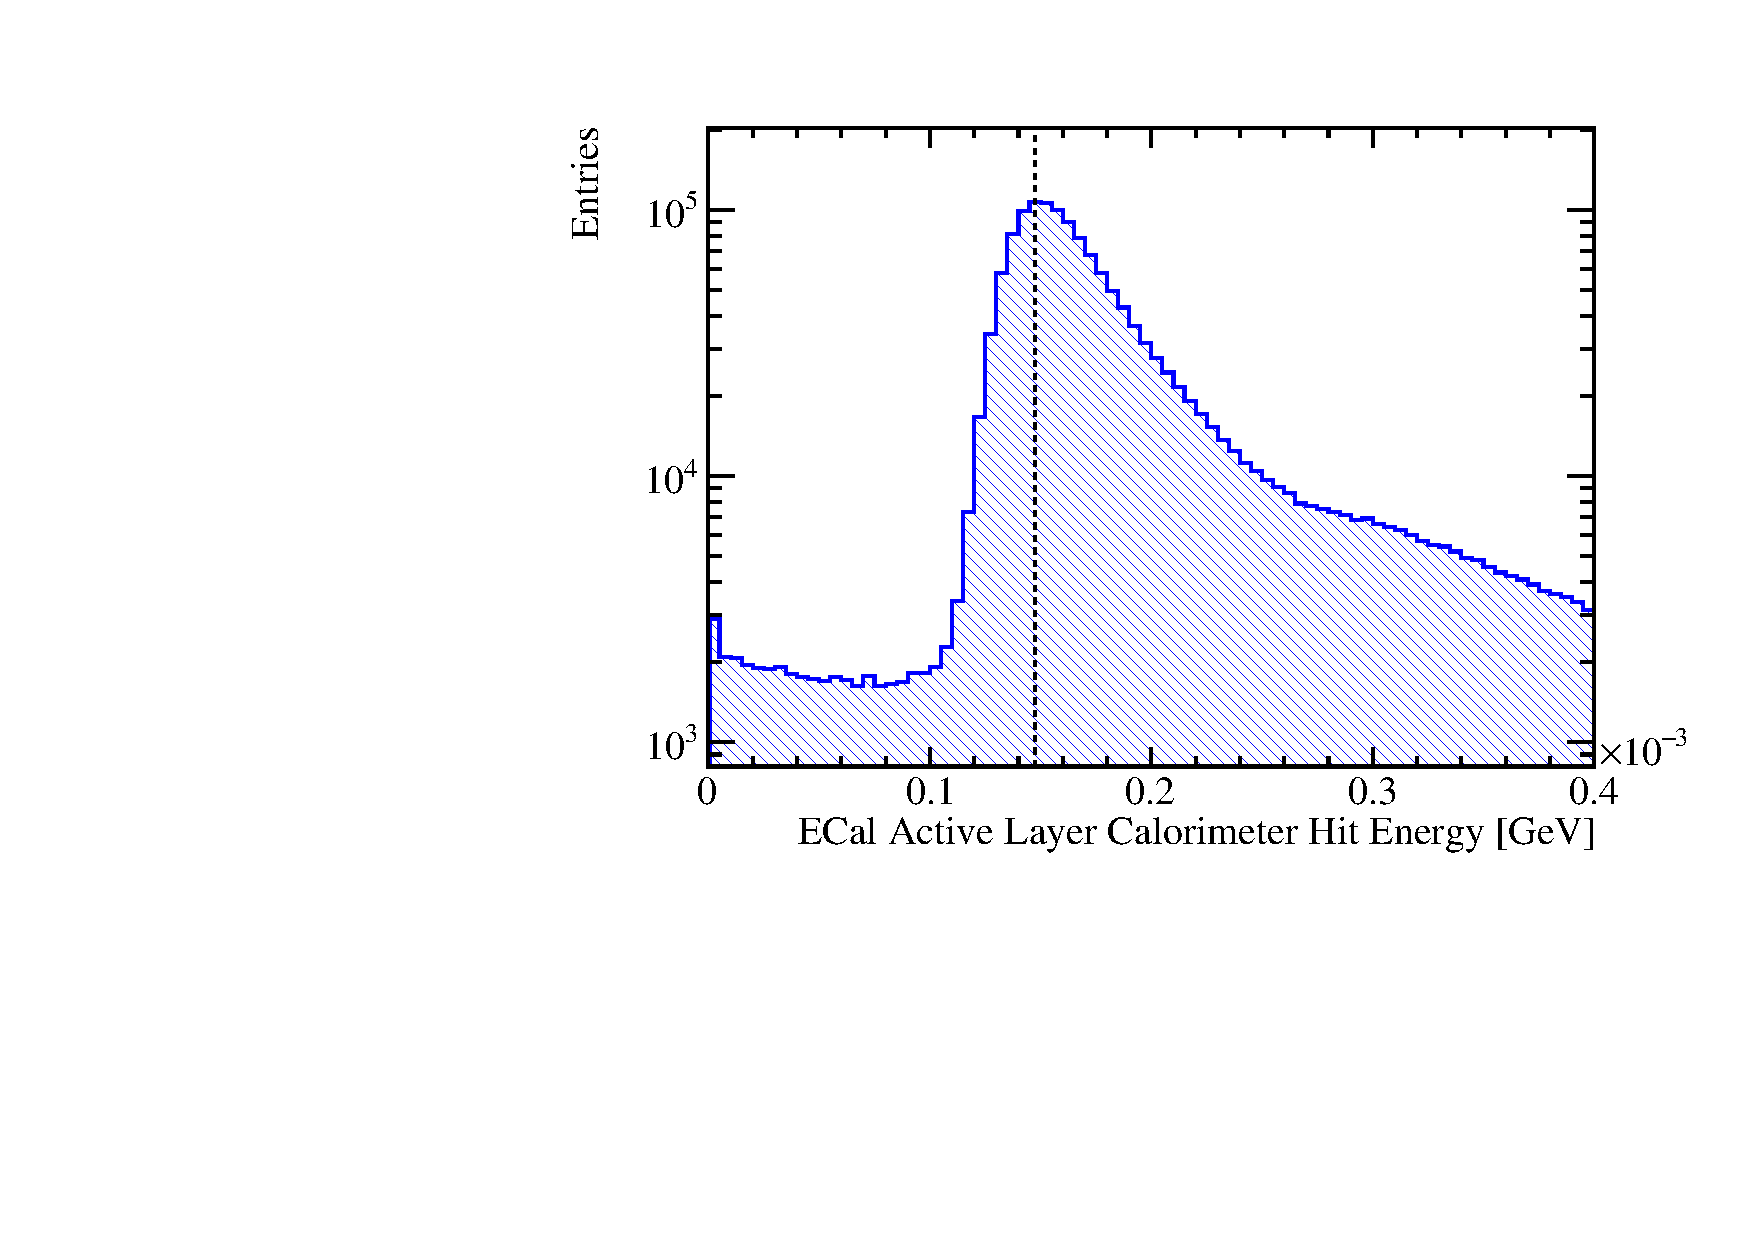
\includegraphics[width=0.5\textwidth]{Calibration/Plots/Calibration/MIPScale/Digitiser/MIPScaleDigitiserECal.pdf}}
\subfloat[]{\label{fig:digitisermiphcalbarrel}\includegraphics[width=0.5\textwidth]{Calibration/Plots/Calibration/MIPScale/Digitiser/MIPScaleDigitiserHCalbarrel.pdf}} \\
\subfloat[]{\label{fig:digitisermiphcalendcap}\includegraphics[width=0.5\textwidth]{Calibration/Plots/Calibration/MIPScale/Digitiser/MIPScaleDigitiserHCalendcap.pdf}}
\subfloat[]{\label{fig:digitisermiphcalring}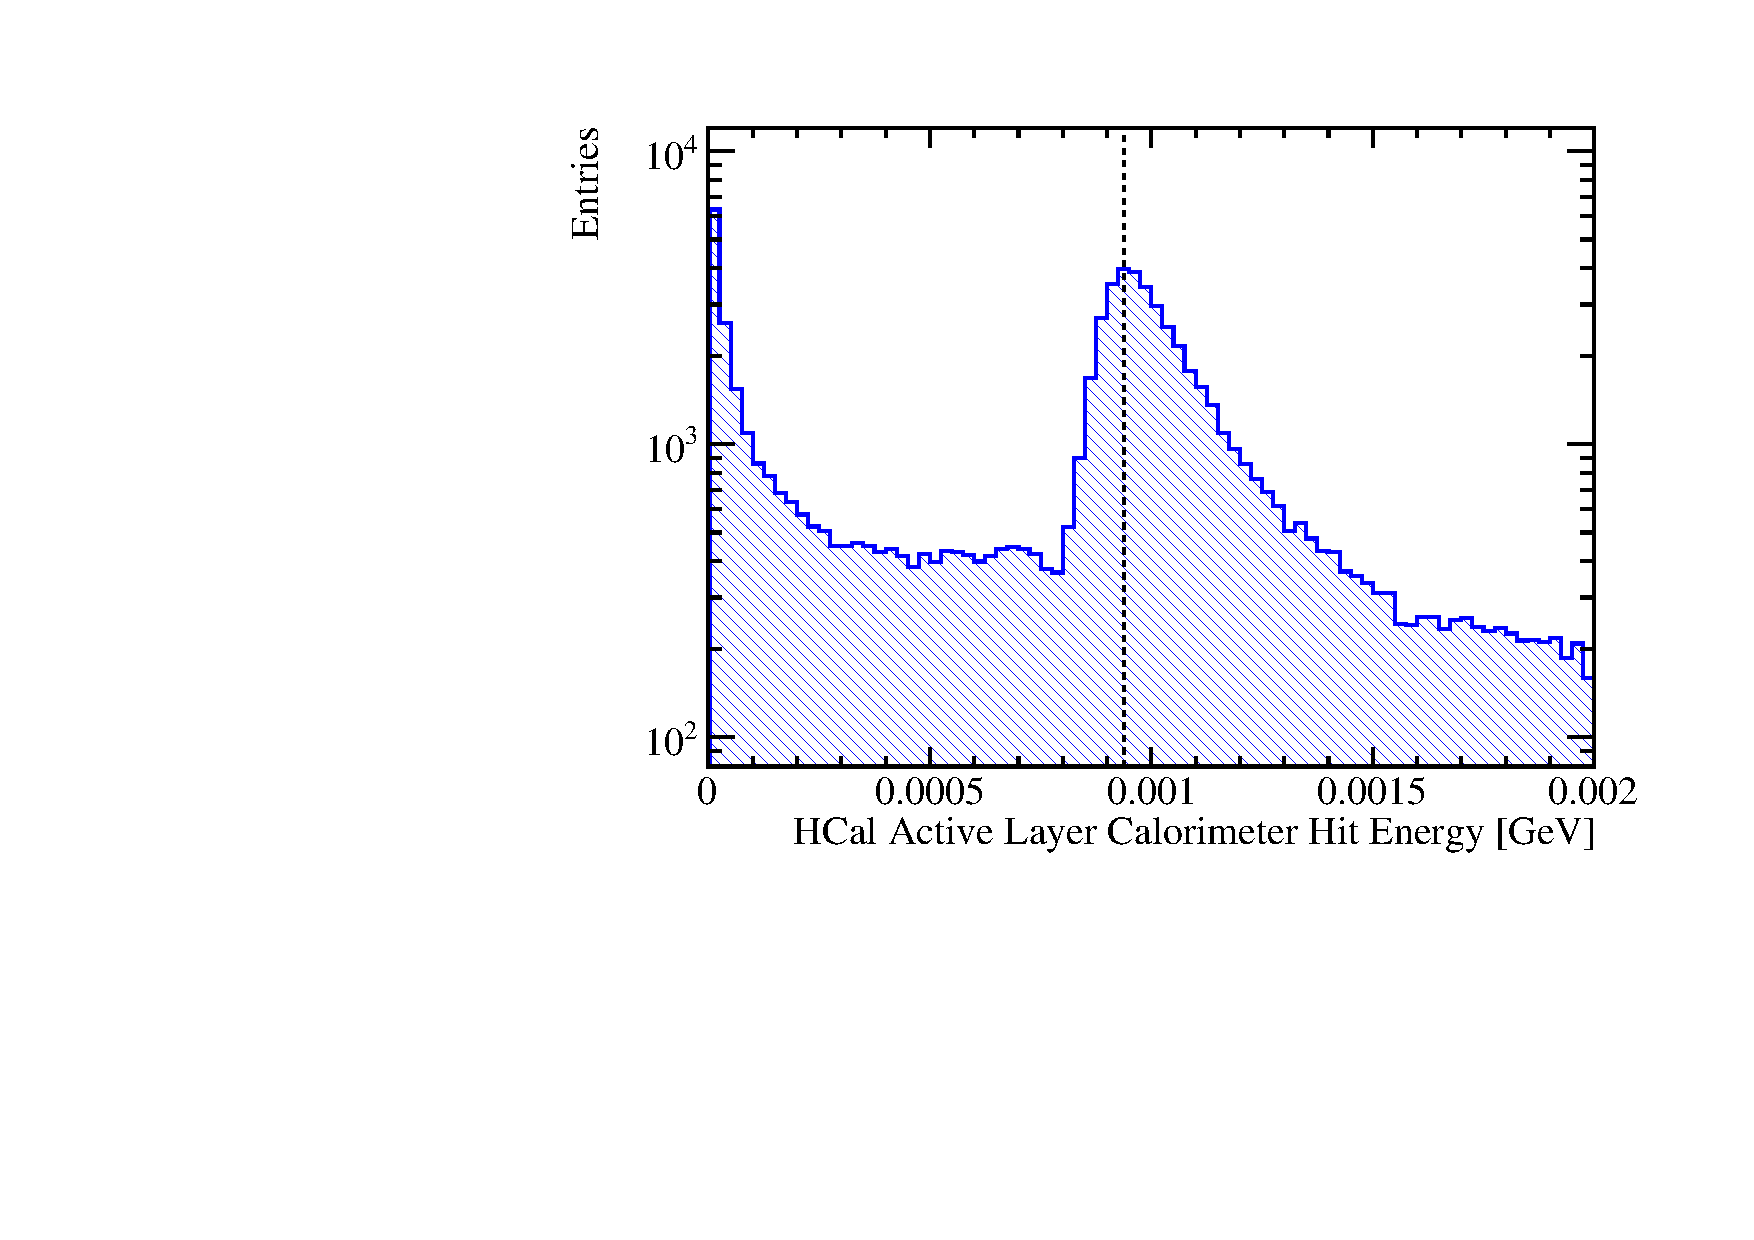
\includegraphics[width=0.5\textwidth]{Calibration/Plots/Calibration/MIPScale/Digitiser/MIPScaleDigitiserHCalOther.pdf}}
\caption[The active layer calorimeter hit energy distributions for \protect\subref{fig:digitisermipecal} the ECal, \protect\subref{fig:digitisermiphcalbarrel} the HCal barrel, \protect\subref{fig:digitisermiphcalendcap} the HCal endcap and \protect\subref{fig:digitisermiphcalring} the HCal ring for 10~GeV $\mu^{-}$ events.  The vertical black dotted lines indicate the position of the MIP peak in these distributions.]{The active layer calorimeter hit energy distributions for \protect\subref{fig:digitisermipecal} the ECal, \protect\subref{fig:digitisermiphcalbarrel} the HCal barrel, \protect\subref{fig:digitisermiphcalendcap} the HCal endcap and \protect\subref{fig:digitisermiphcalring} the HCal ring for 10~GeV $\mu^{-}$ events.  The vertical black dotted lines indicate the position of the MIP peak in these distributions.}
\label{fig:digitisermip}
\end{figure}

%========================================================================================

\subsection{Digitisation Implementation}
\label{sec:digi}
This section discusses how the digitisation constants, $\alpha$s, are determined.  The digitisation constant for a given calorimeter depends upon several factors such as the material properties of the active and absorber layers, the magnetic field strength and energy losses occurring within the gaps in the detector.  Therefore, each calorimeter in the ILD detector model has a distinct constant that must be independently determined. 

%========================================================================================

\subsubsection{ECal Digitisation Implementation}
\label{sec:ecaldigi}
The procedure for determining the digitisation constants in the ECal involves simulation of single photons at an energy $E_{MC} = 10$~GeV.  Single photons at this energy are largely contained within the ECal, as shown in figure \ref{fig:ecaldigiphotonsplit}.  This makes them ideal for isolating the ECal digitisation calibration from that of the HCal digitisation calibration.  Events are only used for calibrating the ECal digitisation if they are confined to the ECal.  To that extent, cuts are applied ensuring that the sum of the reconstructed energy found outside the ECal is less than 1\% of $E_{MC}$ and that the $\text{cos}(\theta) < 0.95$, where $\theta$ is the polar angle of the photon.  Photons that convert are also vetoed in this event sample at MC level.  The impact of these cuts on the sum of ECal hit energies for the $E_{MC} = 10$~GeV photons is shown in figure \ref{fig:ecaldigiselection}.

\begin{figure}[h!]
\subfloat[]{\label{fig:ecaldigiphotonsplit}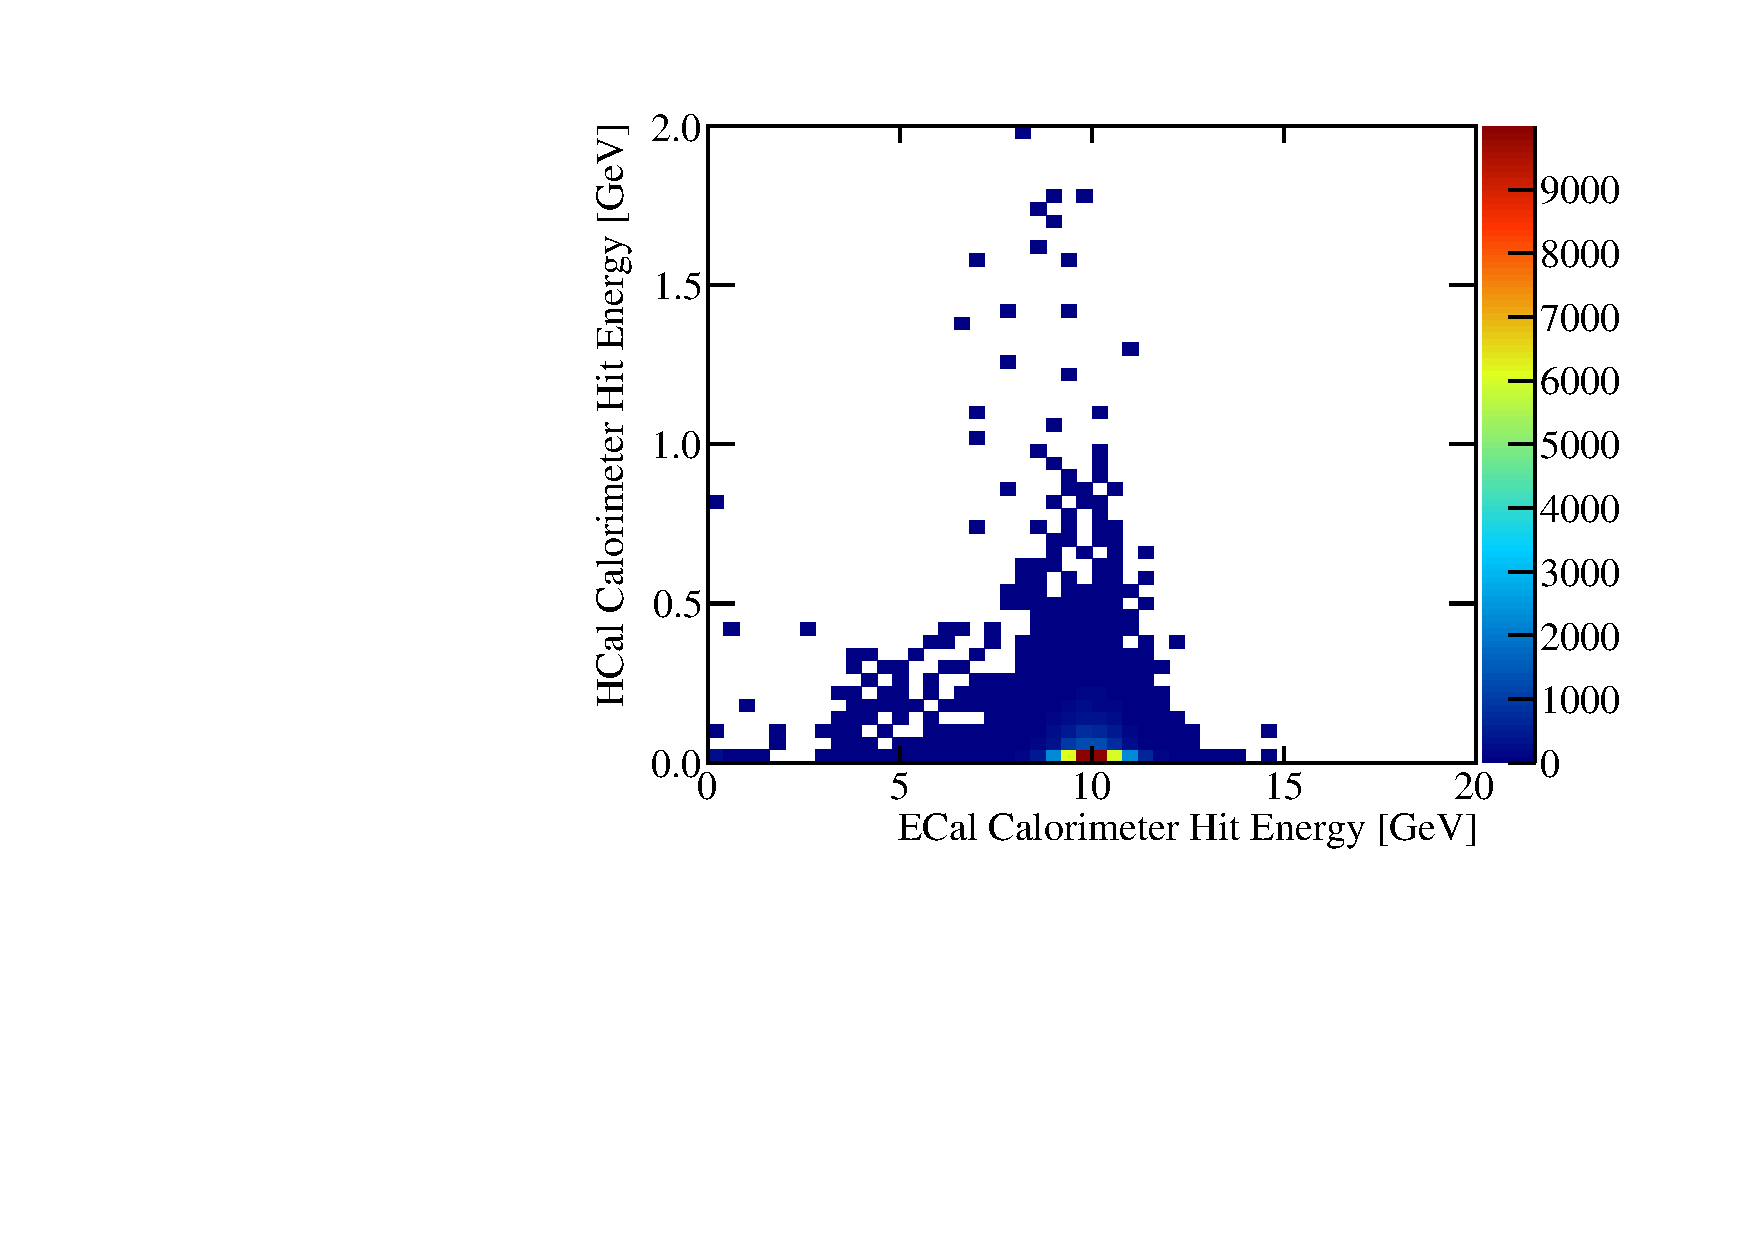
\includegraphics[width=0.5\textwidth]{Calibration/Plots/Calibration/Digitsation/ECal/ECalHCalPhotonSplit.pdf}}
\subfloat[]{\label{fig:ecaldigiselection}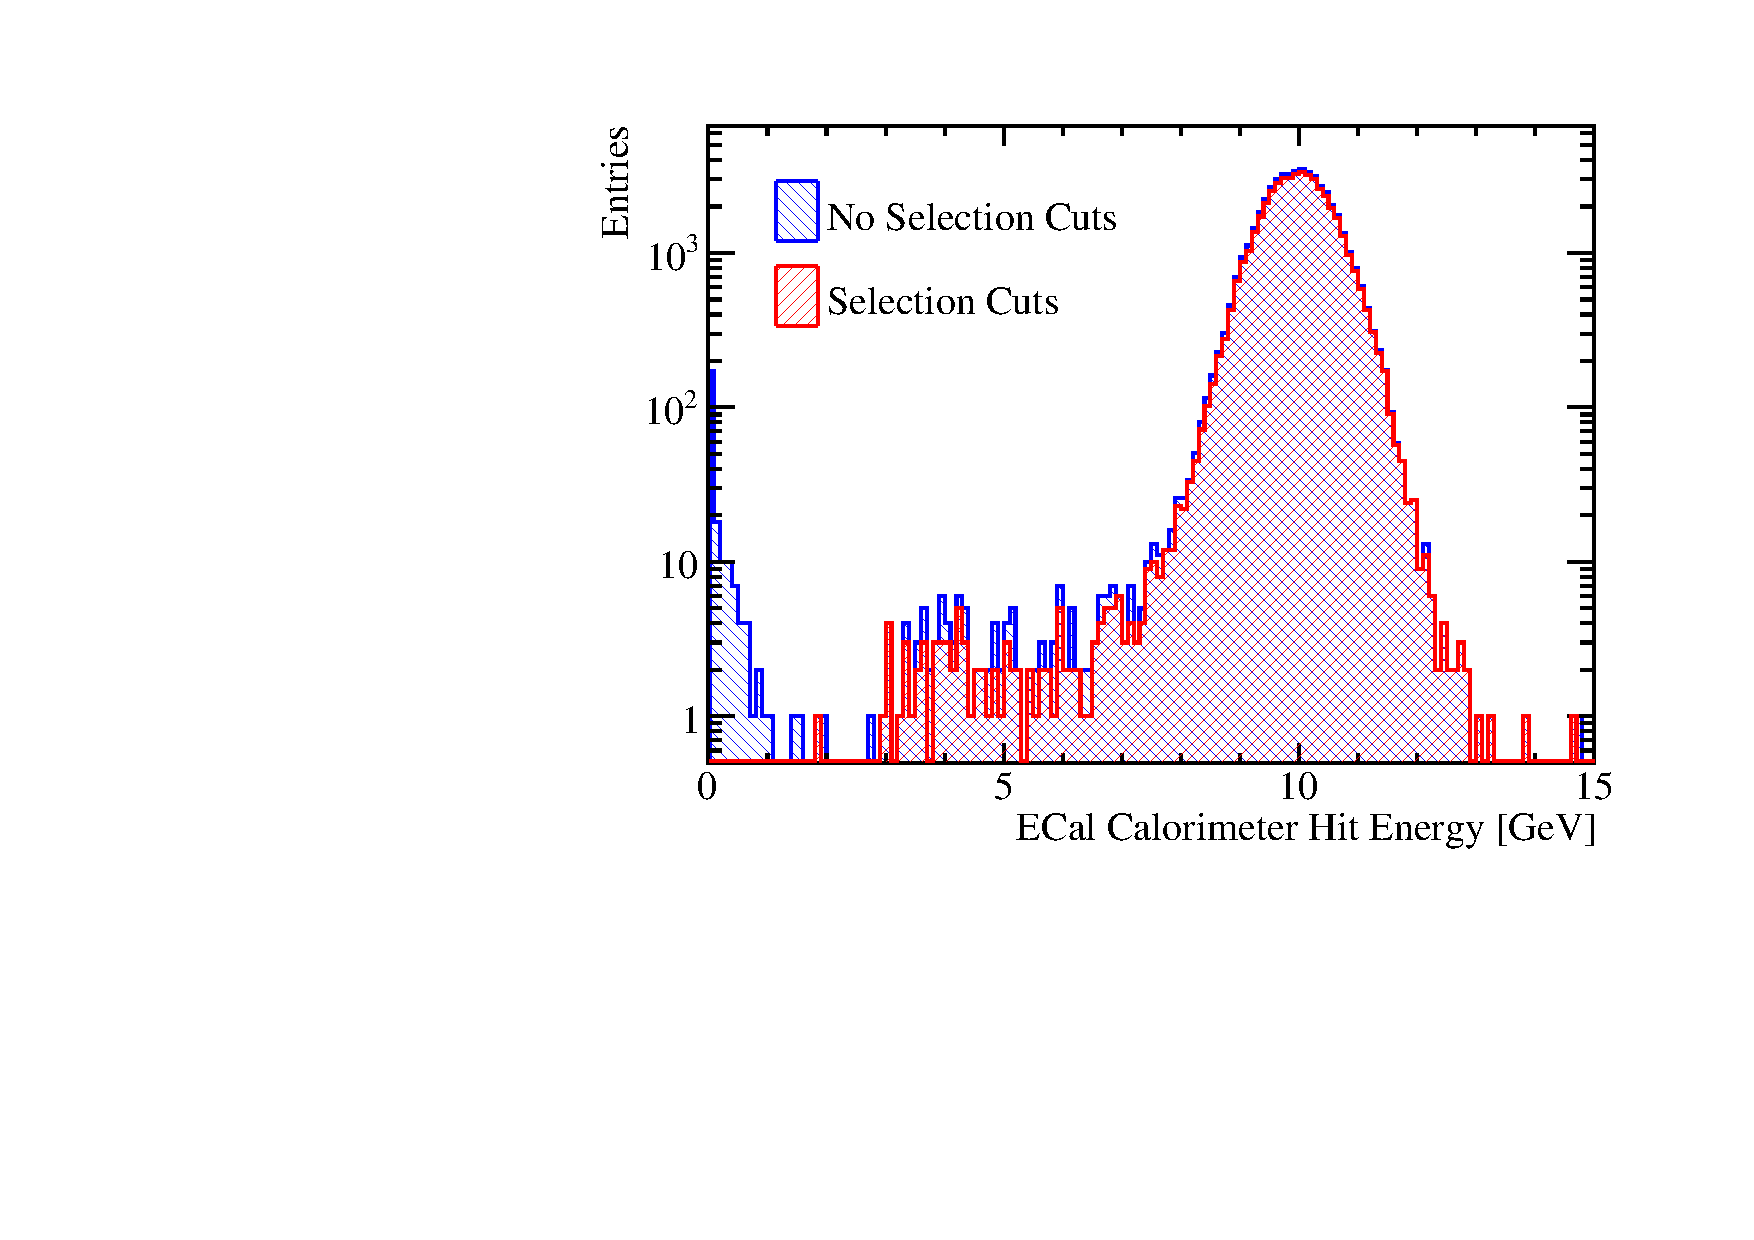
\includegraphics[width=0.5\textwidth]{Calibration/Plots/Calibration/Digitsation/ECal/DigitisationECalSelection.pdf}}
\caption[\protect\subref{fig:ecaldigiphotonsplit} The sum of calorimeter hit energies in ECal and HCal for 10~GeV photons.  \protect\subref{fig:ecaldigiselection} The sum of the ECal calorimeter hit energies for 10~GeV photons with and without the selection cuts.]{\protect\subref{fig:ecaldigiphotonsplit} The sum of calorimeter hit energies in ECal and HCal for 10~GeV photons.  \protect\subref{fig:ecaldigiselection} The sum of the ECal calorimeter hit energies for 10~GeV photons with and without the selection cuts.}
\label{fig:ecaldigi}
\end{figure}

The calibration of the digitisation in the ECal is an iterative procedure, which begins with the simulation of single photons using a trial calibration, $\alpha^{0}_{\text{ECal}}$.  Next the distribution of the sum of calorimeter hit energies within the ECal is produced for events passing the selection cuts, as shown in figure \ref{fig:ecaldigiselection}.  For an ideal calorimeter this distribution should be Gaussian, as described in chapter \ref{chap:detopt}, therefore, a Gaussian fit is applied to this distribution and the mean, $E_{\text{Fit}}$, extracted.  To remove the effect of any outliers in this distribution, the fit is applied to the range of data with the smallest root mean square that contains at least 90 \% of the data.  An example of such a fit is shown in figure \ref{fig:ecaldigifit}.  In the case of ideal calibration, the mean of this fit, $E_{\text{Fit}}$, would be equal $E_{MC}$.  It is assumed that any difference between the two is due to the calibration, therefore, to correct this the digitisation constant from the trial calibration, $\alpha^{0}_{\text{ECal}}$, is rescaled by the ratio of the $E_{MC}$ to $E_{\text{Fit}}$
%
\begin{equation}
\alpha^{0}_{\text{ECal}} \rightarrow \alpha_{\text{ECal}} = \alpha^{0}_{\text{ECal}} \times \frac{E_{MC}}{E_{Fit}}\text{ .}
\end{equation}
%
This procedure is then repeated until the $E_{\text{Fit}}$ falls within a specified tolerance of $E_{MC}$.  The tolerance applied here was $|E_{\text{Fit}} - E_{\text{MC}}| < E_{\text{MC}} \times 5 \%$.  The binning used for the fitted histogram is chosen such that the bin width is equal to the desired tolerance on $E_{\text{Fit}}$ e.g. $E_{\text{MC}} \times 5 \% = 0.5$~GeV.  It should be emphasised that the PFO energies used for downstream analyses have the electromagnetic and hadronic energy scale corrections applied, which are calibrated to a much tighter accuracy.

\begin{figure}[h!]
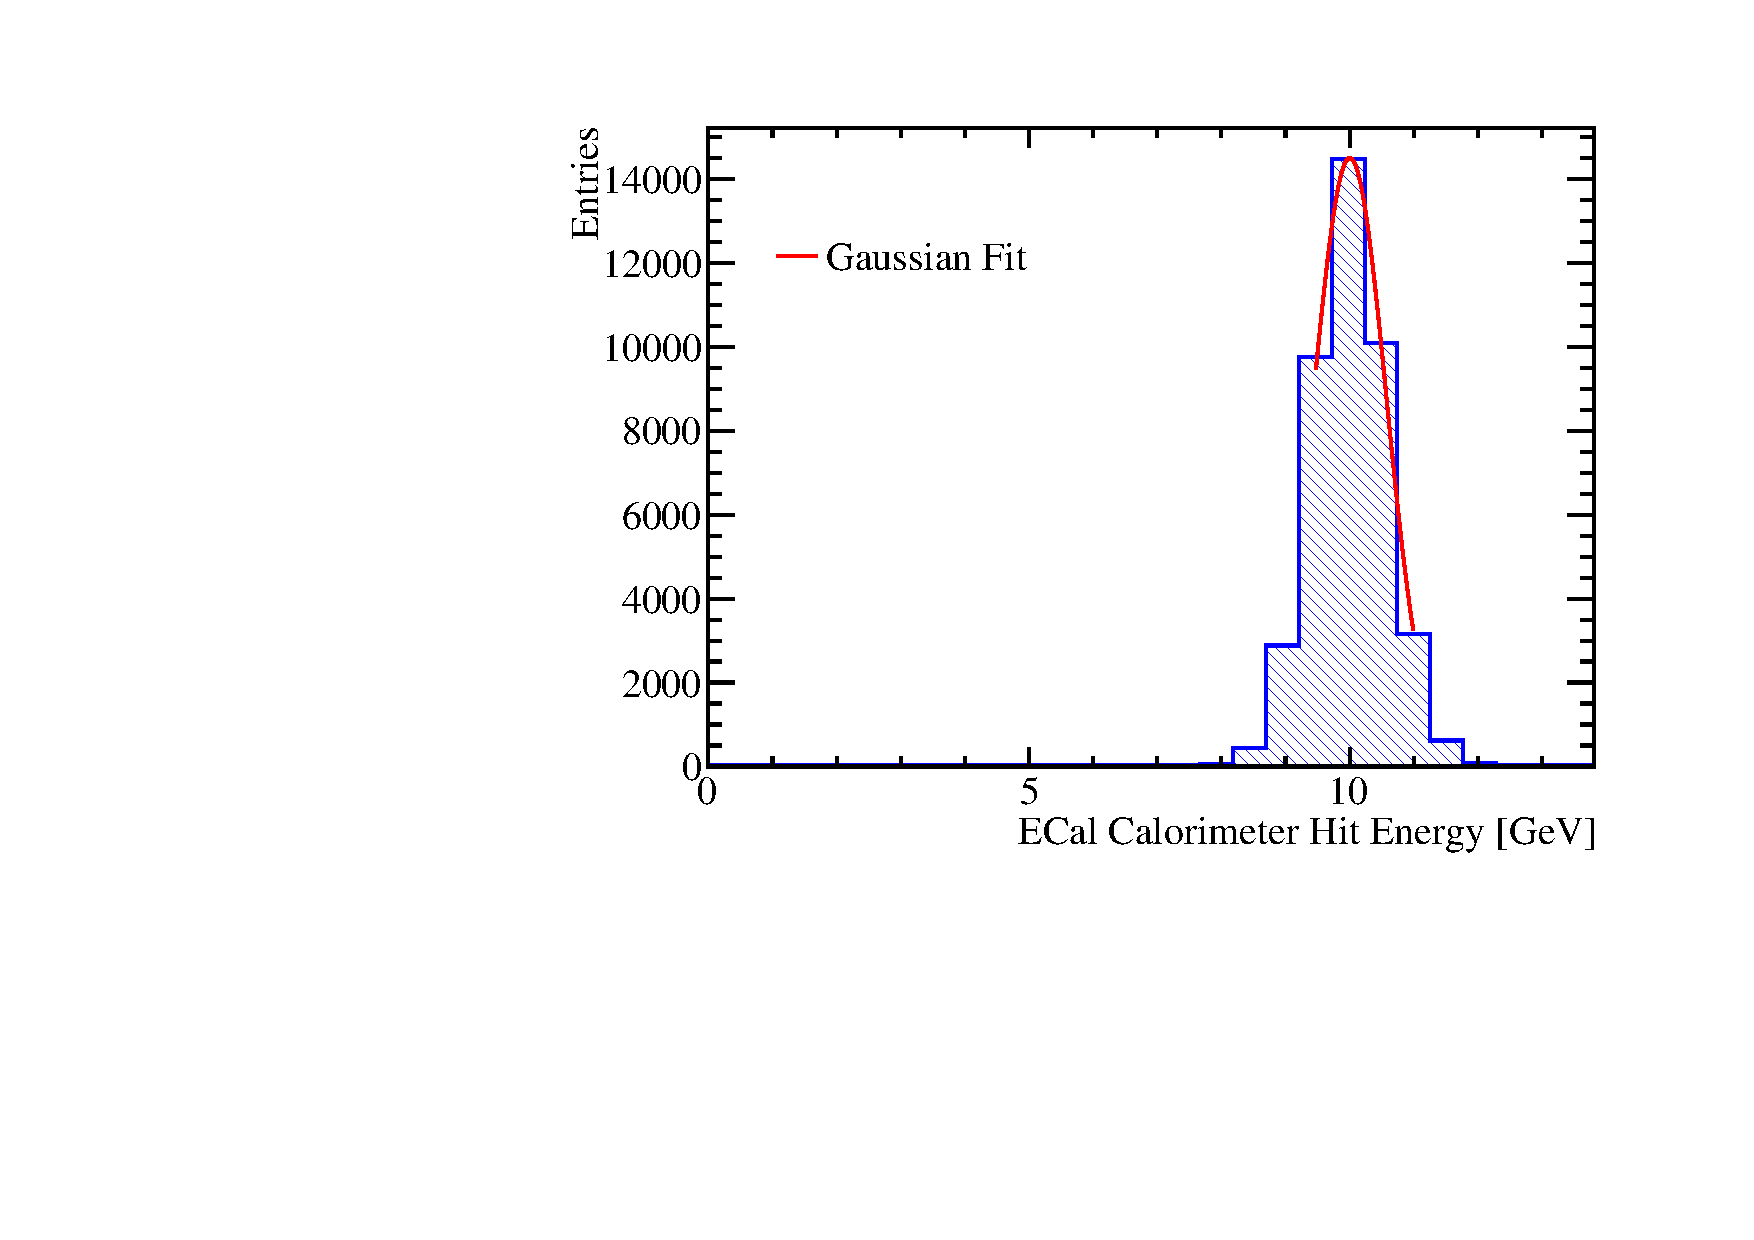
\includegraphics[width=0.5\textwidth]{Calibration/Plots/Calibration/Digitsation/ECal/DigitisationECalFit.pdf}
\caption[Gaussian fit to sum of the ECal calorimeter hit energies for 10~GeV photons with selection cuts.  The coarse binning reflects the tolerance on the digitisation constant calibration.]{Gaussian fit to sum of the ECal calorimeter hit energies for 10~GeV photons with selection cuts.  The coarse binning reflects the tolerance on the digitisation constant calibration.}
\label{fig:ecaldigifit}
\end{figure}

%========================================================================================
% 7467 out of 50000 have no ECal energy. ~ 15 %.  Negligible beampipe evts.

\subsubsection{HCal Digitisation Implementation}
\label{sec:hcaldigi}
The calibration for the digitisation in the HCal proceeds in a similar manner to that described for the ECal with a few key differences.  This calibration uses simulated MC long-lived neutral kaons ($K^{0}_{L}$s) at $E_{MC} = 20$~GeV.  The higher energy, with respect to the ECal digitisation, results in particle showers that sample deeper into the HCal.  The $K^{0}_{L}$s must pass through the ECal, which contains one $\lambda_{I}$, before arriving at the HCal.  Consequently, approximately 15\% of these events begin showering in the ECal, as can be seen in figure \ref{fig:hcaldigikaonsplit}.  Only events that deposit less than 5\% of their energy in the ECal are used for calibrating the HCal digitisation constants.  Furthermore, events that are not contained in the HCal are removed by requiring the last layer of the HCal where energy is deposited is required to be in the innermost 90\% of the HCal.  The impact of these cuts on the sum of HCal calorimeter hit energies for the $E_{MC} = 20$~GeV $K^{0}_{L}$ events is shown in figure \ref{fig:hcaldigiselection}.  

There are two HCal digitisation constants used in the detector simulation, one applied for the barrel and another for the endcap.  The use of two digitisation constants accounts for differences in hadronic shower dynamics between the two, such as differing magnetic field configurations in the barrel and endcap.  Both parameters are calibrated in the same manner, but have different cuts on $\theta$, the polar angle of the $K^{0}_{L}$.  For the barrel region of the HCal events are selected if $0.2 < \text{cos}(\theta) < 0.6$, while for the endcap events are selected if $0.8 < \text{cos}(\theta) < 0.9$.  These angular cuts account for the transverse profile of the hadronic showers and ensure that the showers are largely confined to the relevant sub-detector.  As the majority of the neutral hadrons appearing in jets are neutrons and their accessible energy is the kinetic energy as opposed to the total energy, the target reconstructed energy for these $K^{0}_{L}$ samples is the kinetic energy.  

\begin{figure}[h!]
\subfloat[]{\label{fig:hcaldigikaonsplit}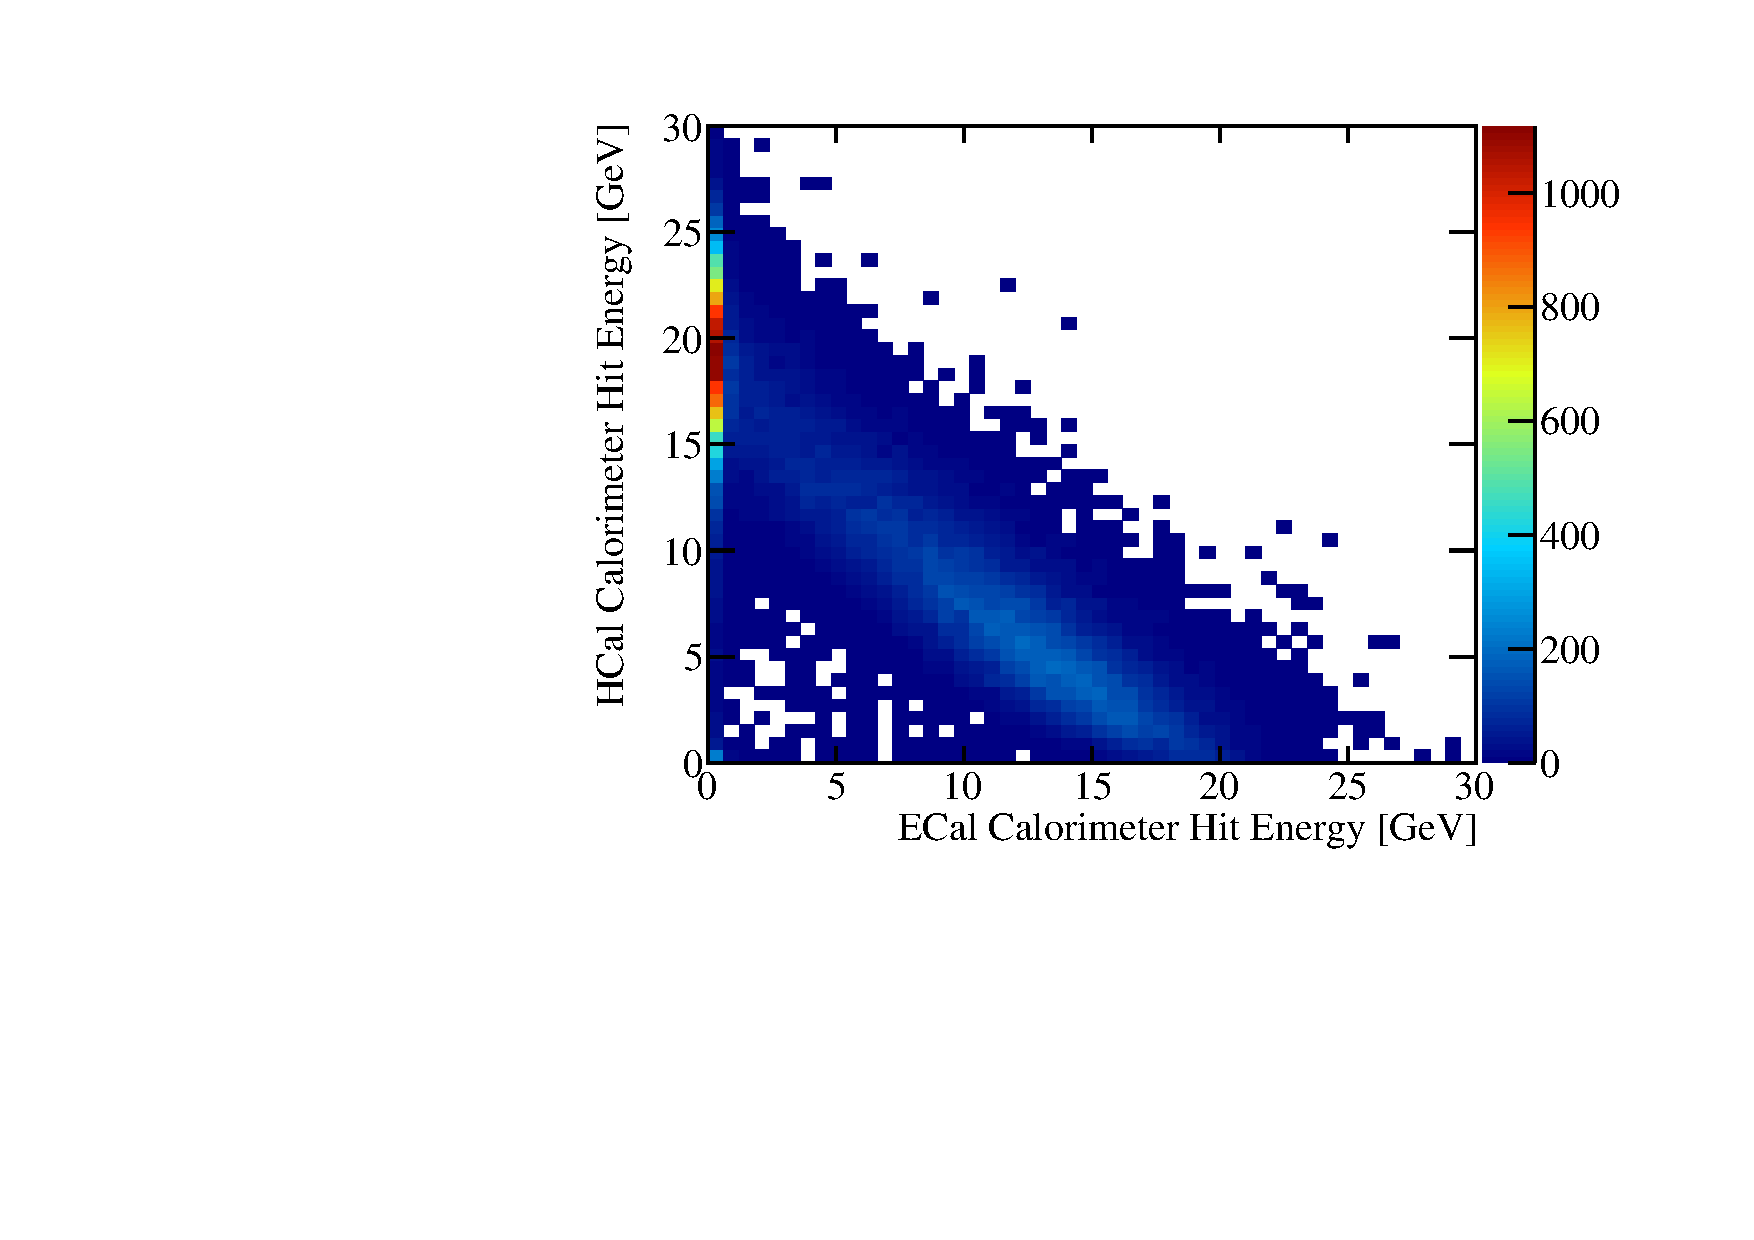
\includegraphics[width=0.5\textwidth]{Calibration/Plots/Calibration/Digitsation/HCal/ECalHCalKaon0LSplit.pdf}}
\subfloat[]{\label{fig:hcaldigiselection}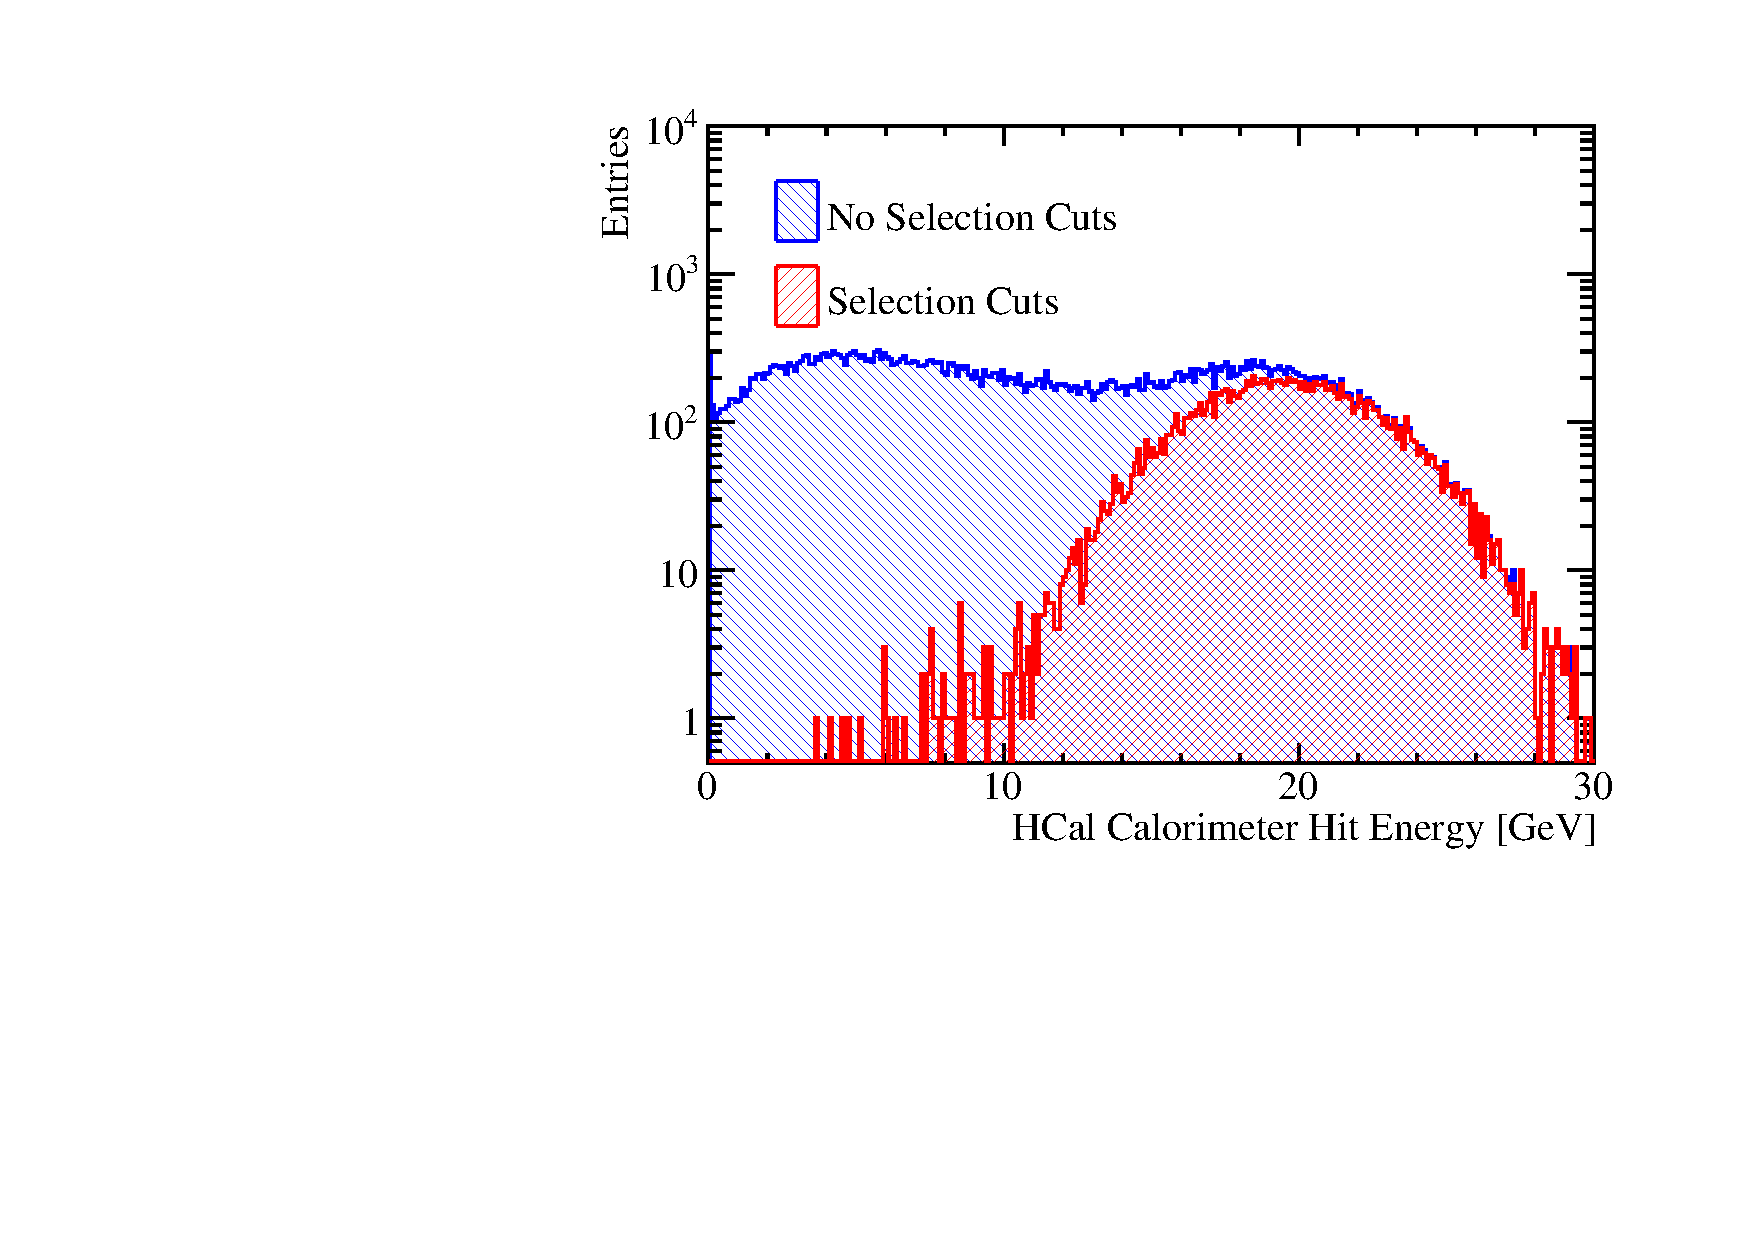
\includegraphics[width=0.5\textwidth]{Calibration/Plots/Calibration/Digitsation/HCal/DigitisationHCalSelection.pdf}}
\caption[\protect\subref{fig:hcaldigikaonsplit} Sum of calorimeter hit energies in ECal and HCal for 20~GeV $K^{0}_{L}$ events.  \protect\subref{fig:hcaldigiselection} Sum of the HCal calorimeter hit energies for a 20~GeV $K^{0}_{L}$ events with and without the selection cuts.]{\protect\subref{fig:hcaldigikaonsplit} Sum of calorimeter hit energies in ECal and HCal for 20~GeV $K^{0}_{L}$ events.  \protect\subref{fig:hcaldigiselection} Sum of the HCal calorimeter hit energies for a 20~GeV $K^{0}_{L}$ events with and without the selection cuts.}
\label{fig:hcaldigi}
\end{figure}

After applying the above $K^{0}_{L}$ selection cuts, the calibration procedure for the digitisation of the HCal barrel and endcap proceeds in the same manner as was described for the ECal.  An example of the Gaussian fits applied to the sum of the calorimeter hit energies in the HCal barrel and endcap are shown in figure \ref{fig:hcaldigifit}.  

\begin{figure}[h!]
\subfloat[HCal barrel.]{\label{fig:hcaldigibarrel}\includegraphics[width=0.5\textwidth]{Calibration/Plots/Calibration/Digitsation/HCal/DigitisationHCalbarrelFit.pdf}}
\subfloat[HCal endcap.]{\label{fig:hcaldigiendcap}\includegraphics[width=0.5\textwidth]{Calibration/Plots/Calibration/Digitsation/HCal/DigitisationHCalendcapFit.pdf}}
\caption[Gaussian fit to sum of the HCal calorimeter hit energies for 20~GeV $K^{0}_{L}$ events with selection cuts.]{Gaussian fit to sum of the HCal calorimeter hit energies for 20~GeV $K^{0}_{L}$ events with selection cuts.}
\label{fig:hcaldigifit}
\end{figure}

%========================================================================================

\subsubsection{HCal Ring Digitisation Implementation}
\label{sec:hcalringdigi}
The HCal ring, as illustrated in figure \ref{fig:calorimeters}, is a hadronic calorimeter that surrounds the ECal endcap and is sandwiched between the HCal barrel and endcap.  This calorimeter is required to ensure hermetic coverage of the hadronic calorimeter system across the barrel/endcap cross-over region \cite{Behnke:2013lya}.  

The HCal ring has an independent digitisation constant to account for any difference in the hadronic shower development between the ring, barrel and endcap.  Due to the thickness of the HCal ring, particle showers are never fully contained in it, so a different approach to calibration is required.  To ensure that the HCal ring calibration is approximately correct, $\alpha_{\text{HCal ring}}$ is assumed to equal $\alpha_{\text{HCal endcap}}$ multiplied by several factors designed to account for differences in the active layer thickness, absorber layer thickness and the MIP response between the HCal endcap and ring.  In detail
%
\begin{equation}
\alpha_{\text{HCal ring}} = \alpha_{\text{HCal endcap}} \times \frac{\langle \text{cos}(\theta_\text{endcap}) \rangle}{\langle \text{cos}(\theta_\text{ring}) \rangle} \times \frac{P_\text{endcap} }{P_\text{ring} } \times \frac{L^{Absorber}_\text{endcap}}{L^{Absorber}_\text{ring} } \times \frac{L^{Active}_\text{ring}}{L^{Active}_\text{endcap}} \text{ ,}
\end{equation}
%
\noindent where $\theta$ is the incident angle of the incoming particle to the calorimeter determined using the 20~GeV $K^{0}_{L}$s, $L^{Active}$ is the active layer thickness and $L^{Absorber}$ is the absorber layer thickness.  $P$ is the position of the MIP peak in the distribution of active layer hit energies, which has been corrected so that the MIP appears to enter the calorimeter at normal incidence, and is determined using 10~GeV $\mu^{-}$ events.  Details on how $P$ is determined are given in section \ref{sec:mipresponse}.

\begin{figure}[h!]
\subfloat[]{\label{fig:ecal}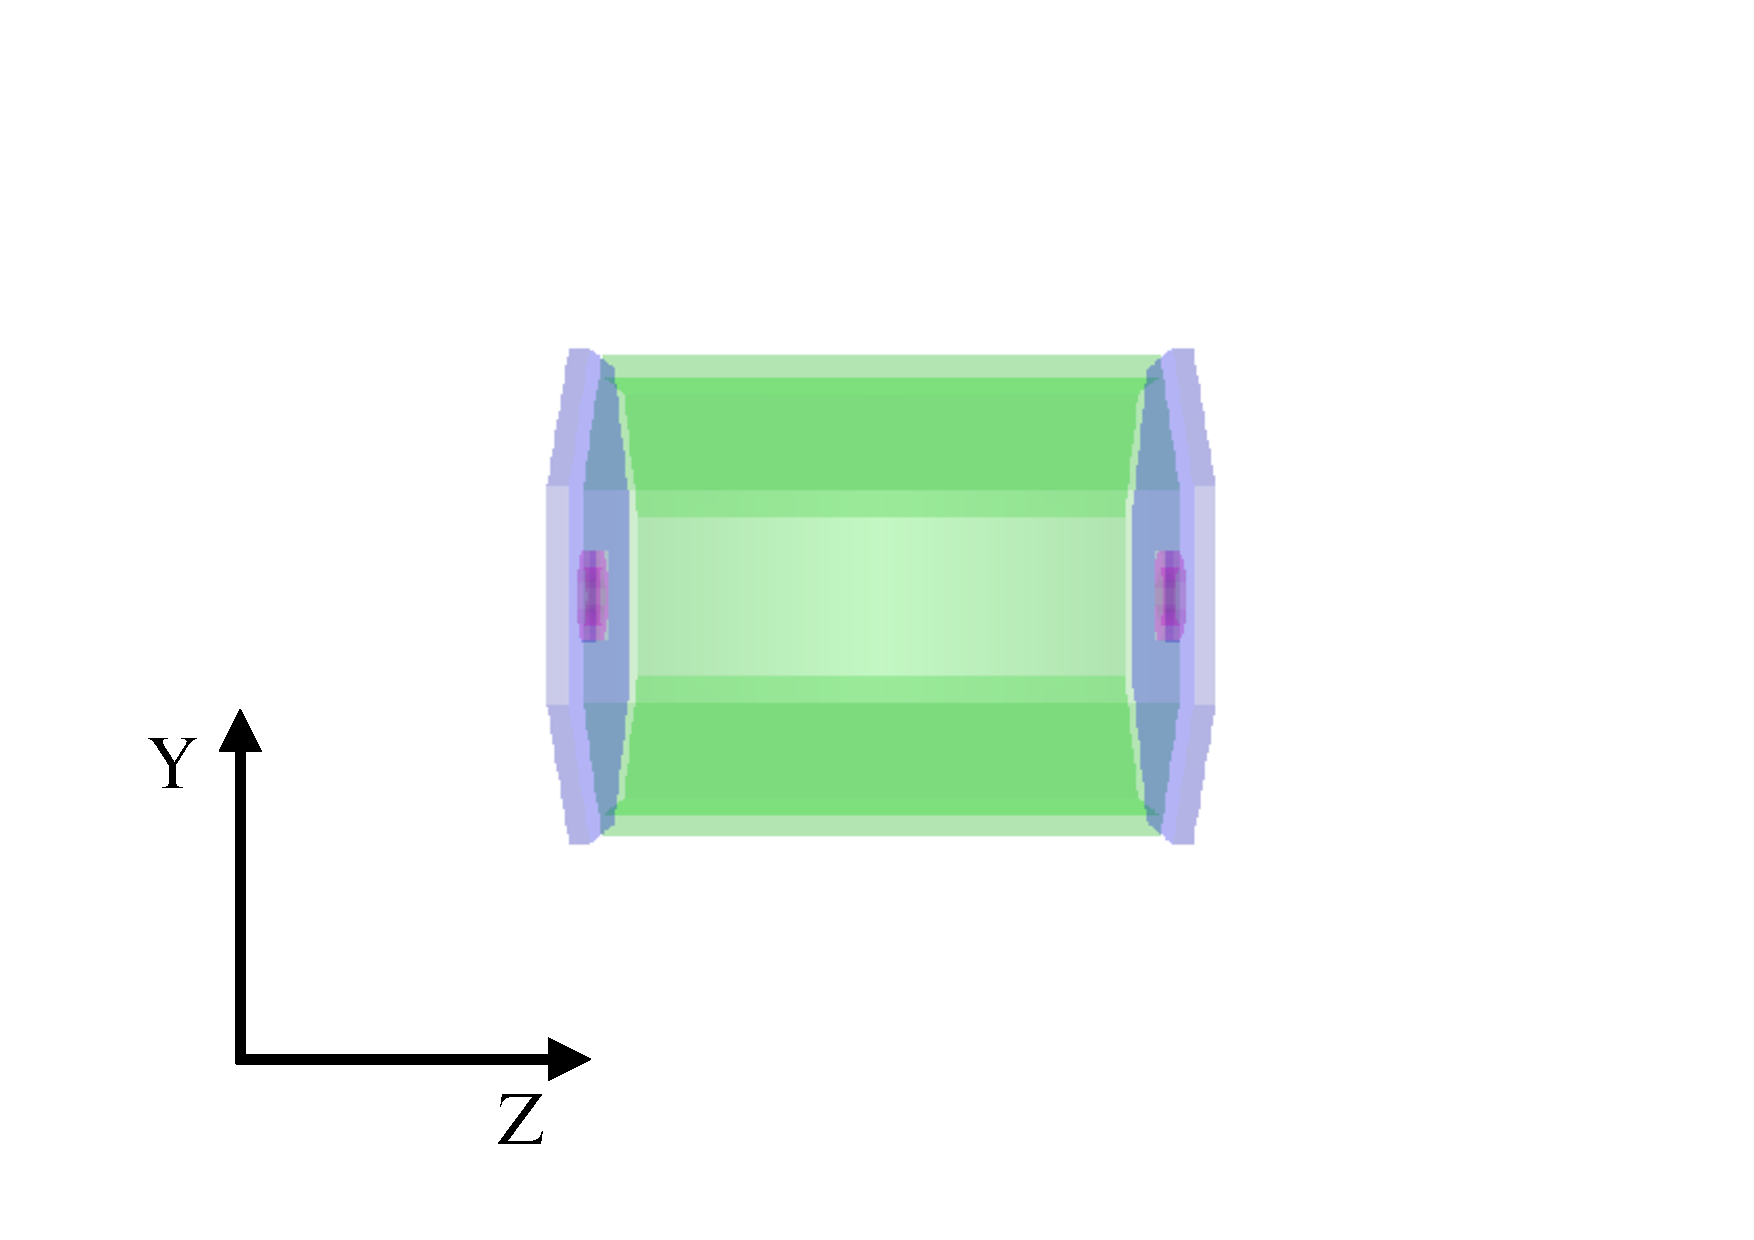
\includegraphics[width=0.33\textwidth]{Calibration/Plots/Calibration/VisualDisplay/ECalWithScale.pdf}}
\subfloat[]{\label{fig:hcal}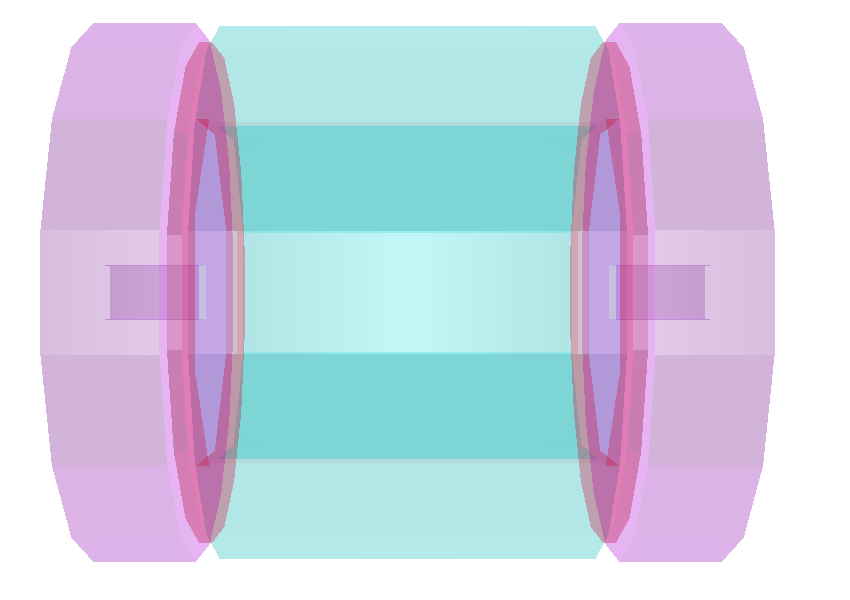
\includegraphics[width=0.33\textwidth]{Calibration/Plots/Calibration/VisualDisplay/HCal.png}}
\subfloat[]{\label{fig:hcalring}\includegraphics[width=0.33\textwidth]{Calibration/Plots/Calibration/VisualDisplay/HCalring.png}}
\caption[A PandoraPFA event display showing the nominal ILD calorimeters.  \protect\subref{fig:ecal} the ECal, \protect\subref{fig:hcal} the full HCal and \protect\subref{fig:hcalring} the HCal ring, which covers the barrel/endcap cross-over region.]{A PandoraPFA event display showing the nominal ILD calorimeters.  \protect\subref{fig:ecal} the ECal, \protect\subref{fig:hcal} the full HCal and \protect\subref{fig:hcalring} the HCal ring, which covers the barrel/endcap cross-over region.}
\label{fig:calorimeters}
\end{figure}

%========================================================================================

\subsection{MIP Scale Determination in PandoraPFA}
A similar procedure was employed for calculation of the MIP peak in PandoraPFA.  The distribution used to set the MIP scale in PandoraPFA is the distribution of the calorimeter hit energies, i.e. the active and absorber layer energies, as opposed to the active layer energies used for setting the MIP scale in the digitisation processor.   Examples of the distributions used to set the MIP scale in PandoraPFA can be found in figure \ref{fig:pandoramip}.  There are few populated low calorimeter hit energy bins in this these distributions as cuts are applied in the digitiser on the active layer energy.  The double peak structure observed in the ECal calorimeter hit energy distribution is expected given the ECal absorber material thickness doubling in the back 10 layers of the ECal.  Further differences between the MIP scale setting in the digitiser and PandoraPFA are as follows: The MIP scale setting in PandoraPFA combines the HCal sub-detectors, the barrel, endcap and ring, together when creating the calorimeter hit energy distributions; PandoraPFA requires the MIP scale to be set in the muon chamber unlike the digitisation processor and, therefore, the muon chamber hit energy distribution must also be created.  

\begin{figure}[h!]
\subfloat[]{\label{fig:pandoramipecal}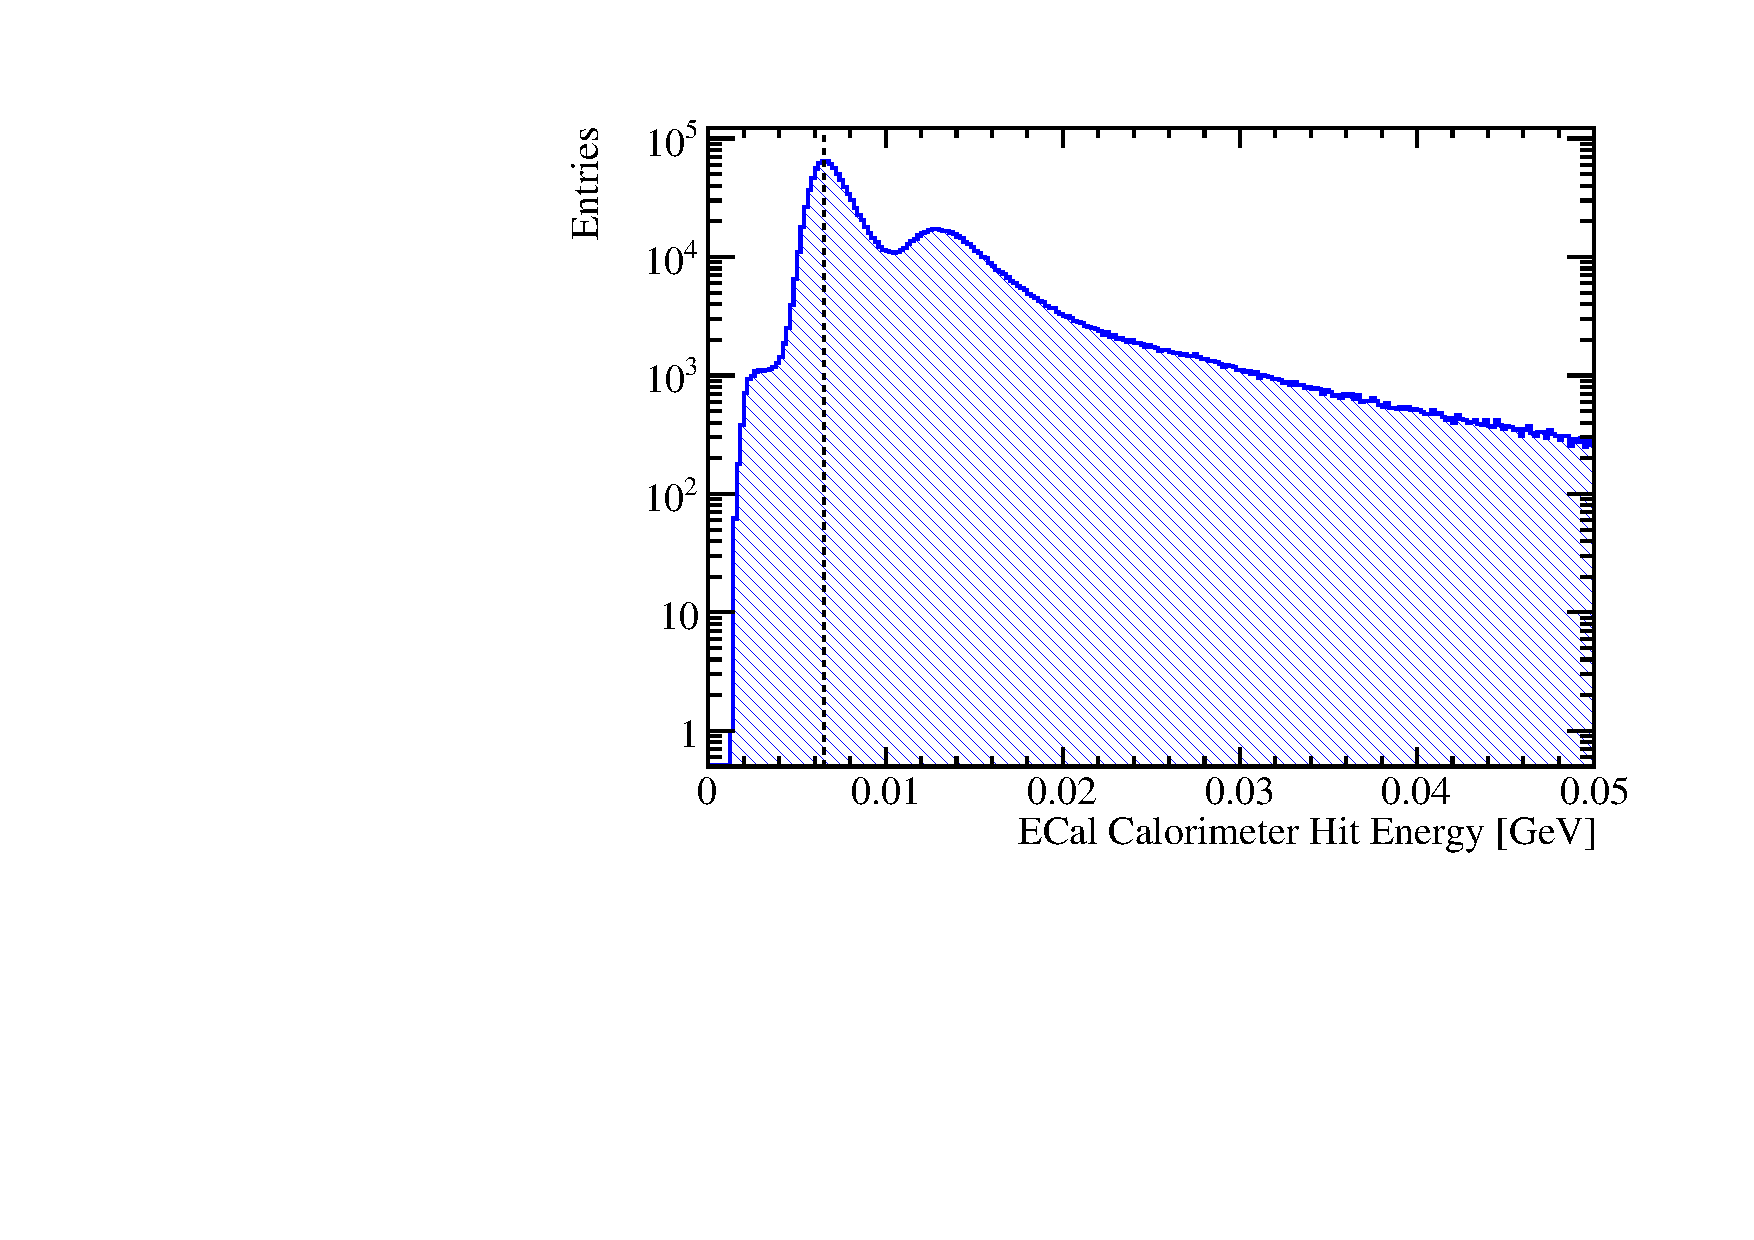
\includegraphics[width=0.5\textwidth]{Calibration/Plots/Calibration/MIPScale/PandoraPFA/MIPScalePandoraPFAECal.pdf}}
\subfloat[]{\label{fig:pandoramiphcal}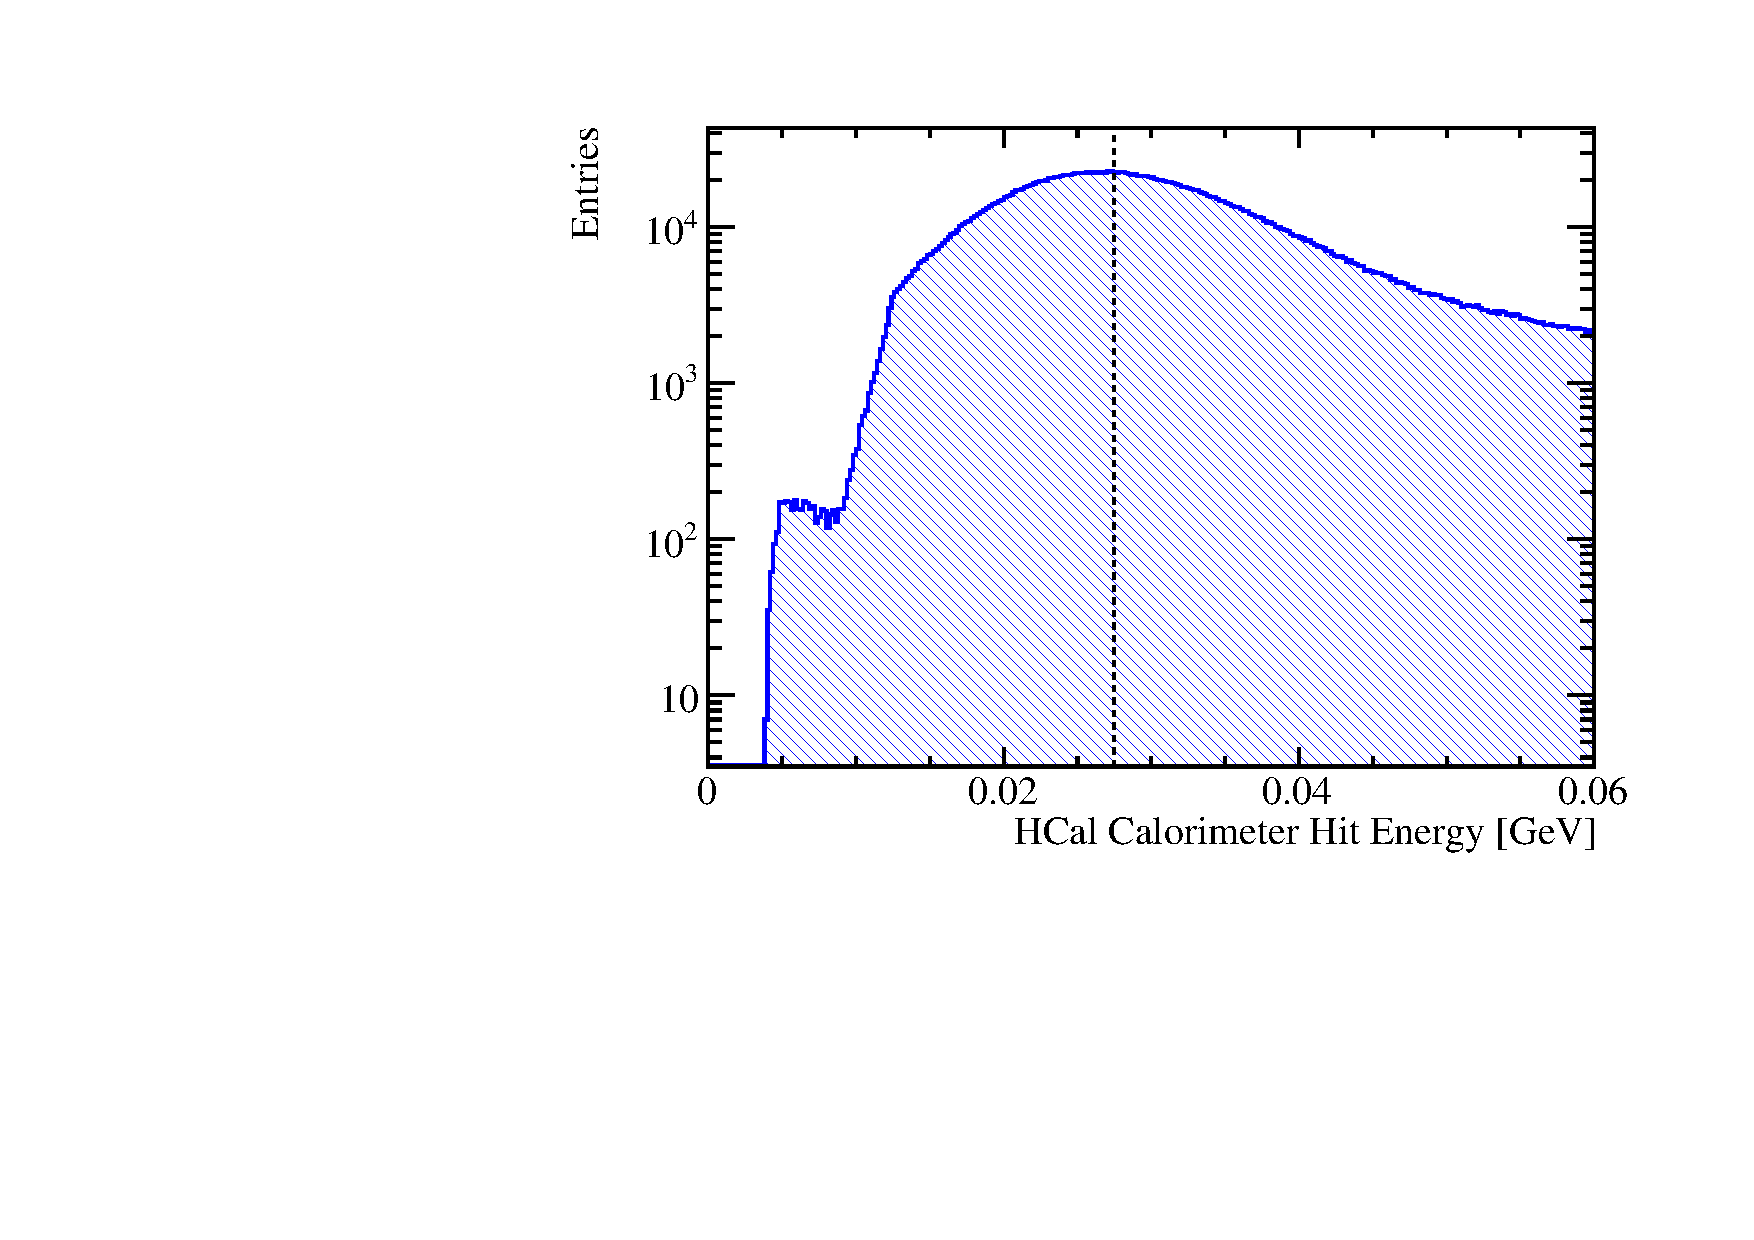
\includegraphics[width=0.5\textwidth]{Calibration/Plots/Calibration/MIPScale/PandoraPFA/MIPScalePandoraPFAHCal.pdf}} \\
\subfloat[]{\label{fig:pandoramipmuon}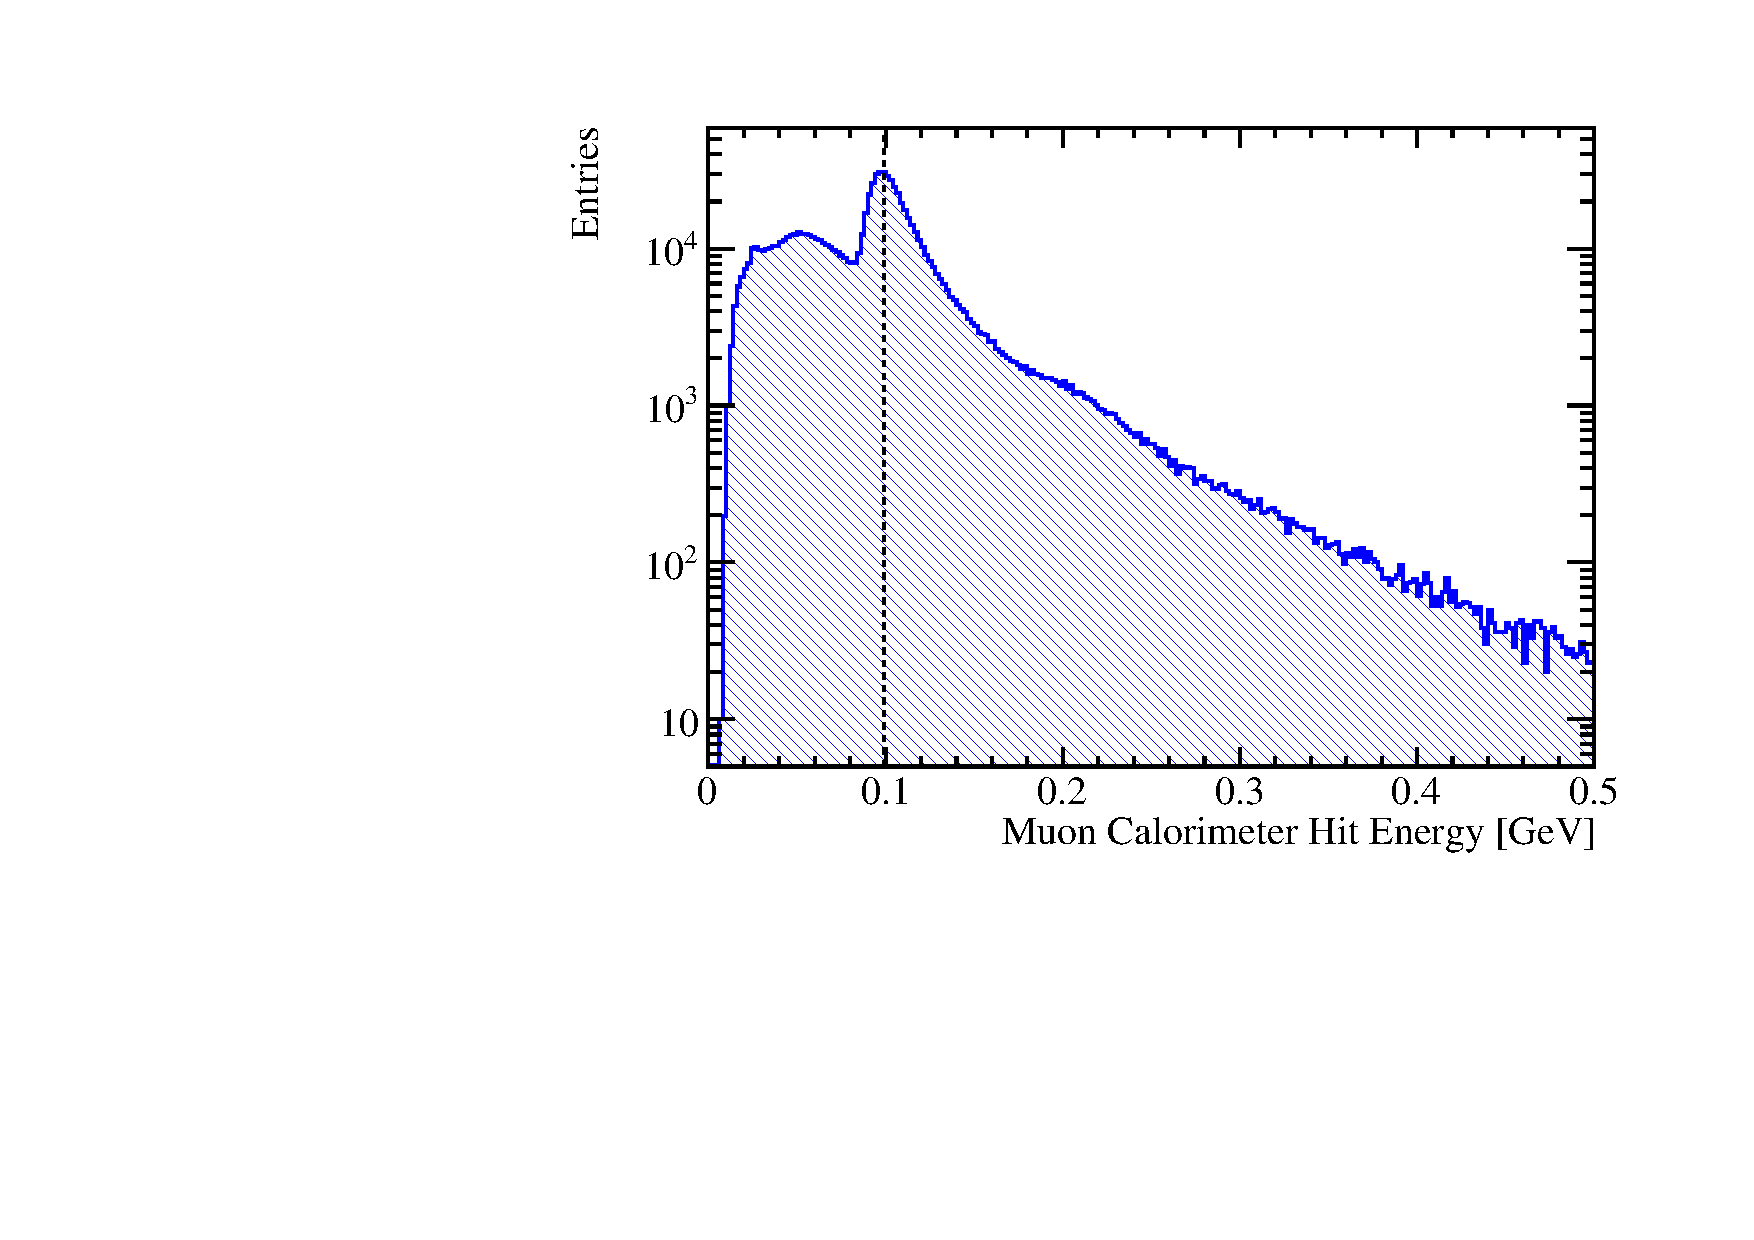
\includegraphics[width=0.5\textwidth]{Calibration/Plots/Calibration/MIPScale/PandoraPFA/MIPScalePandoraPFAMuon.pdf}}
\caption[The calorimeter hit energy distributions for \protect\subref{fig:pandoramipecal} the ECal, \protect\subref{fig:pandoramiphcal} the HCal and \protect\subref{fig:pandoramipmuon} the muon chamber for 10~GeV $\mu^{-}$ events.]{The calorimeter hit energy distributions for \protect\subref{fig:pandoramipecal} the ECal, \protect\subref{fig:pandoramiphcal} the HCal and \protect\subref{fig:pandoramipmuon} the muon chamber for 10~GeV $\mu^{-}$ events.}
\label{fig:pandoramip}
\end{figure}

%========================================================================================

\subsection{Electromagnetic and Hadronic Scale Setting}
\label{sec:scalesetting}

%========================================================================================

\subsubsection{Electromagnetic scale setting}
\label{sec:emscalesetting}
The electromagnetic scale in the ECal, $\beta^{EM}_{ECal}$, is determined using photons at $E_{MC} = 10$~GeV.  Photons are ideal for setting the electromagnetic scale as they procedure electromagnetic showers that are primarily confined to the ECal, which is shown by figure \ref{fig:ecaldigiphotonsplit}.  To ensure that the events used for this part of the calibration are largely confined to the ECal, a cut requiring less than 1\% of the reconstructed energy to be found outside the ECal is applied.  Furthermore, a cut requiring a single $\gamma$ be reconstructed are added to veto events with pattern recognition failures.  $\gamma$ conversions are excluded at MC level to ensure energy measurements used in the calibration arise from the calorimeters and not the charged particle tracks.  The impact of these cuts on the electromagnetic energy measured in the ECal for 10~GeV photons is shown in figure \ref{fig:ecalemscaleselection}.  In figure \ref{fig:ecalemscaleselection}, the peak with zero electromagnetic energy in the ECal is due to events traveling down the beam pipe and events with $\gamma$ conversions.  In $\gamma$ conversion events the reconstructed energy is taken from the $\text{e}^{\pm}$ tracks, which means the electromagnetic energy in the ECal will register as zero.  The tail of events with low electromagnetic energy in the ECal occurs primarily due pattern recognition failures in $\gamma$ conversion events.  In such cases, some of the calorimetric energy deposits are not associated to the $\text{e}^{\pm}$ tracks and instead form new $\gamma$s that contain only a small fraction of the true MC energy.  

The fitting procedure follows that used for the ECal digitisation, described in section \ref{sec:ecaldigi}, whereby a trial calibration for the electromagnetic energy scale in the ECal, $\beta^{EM0}_{ECal}$, is assumed and the single photons simulated.  The distribution of the electromagnetic energy in the ECal is created and a Gaussian fit applied to the range of data with the smallest root mean square containing at least 90 \% of the data.  The mean of this fit, $E_{\text{Fit}}$, is then used to scale $\beta^{EM0}_{ECal}$ in the following way
%
\begin{equation}
\beta^{EM0}_{ECal} \rightarrow \beta^{EM}_{ECal} = \beta^{EM0}_{ECal} \times \frac{E_{MC}}{E_{Fit}}\text{ .}
\end{equation}
%
An example distribution and fit used in the calibration of the nominal ILD detector model can be found in figure \ref{fig:ecalemscalefit}.  This procedure is repeated using the updated $\beta^{EM}_{ECal}$ until $E_{\text{Fit}}$ falls within a specified tolerance.  The tolerance applied here was $|E_{\text{Fit}} - E_{\text{MC}}| < E_{\text{MC}} \times 0.5 \%$.  The binning for the fitted histogram is chosen such that the bin width is equal to the desired target tolerance on $E_{\text{Fit}}$ e.g. $E_{\text{MC}} \times 0.5 \% = 0.05$~GeV.  This tolerance is tighter than was applied for the digitisation as it is these energies that are used in downstream analyses.   
 
\begin{figure}[h!]
\subfloat[]{\label{fig:ecalemscaleselection}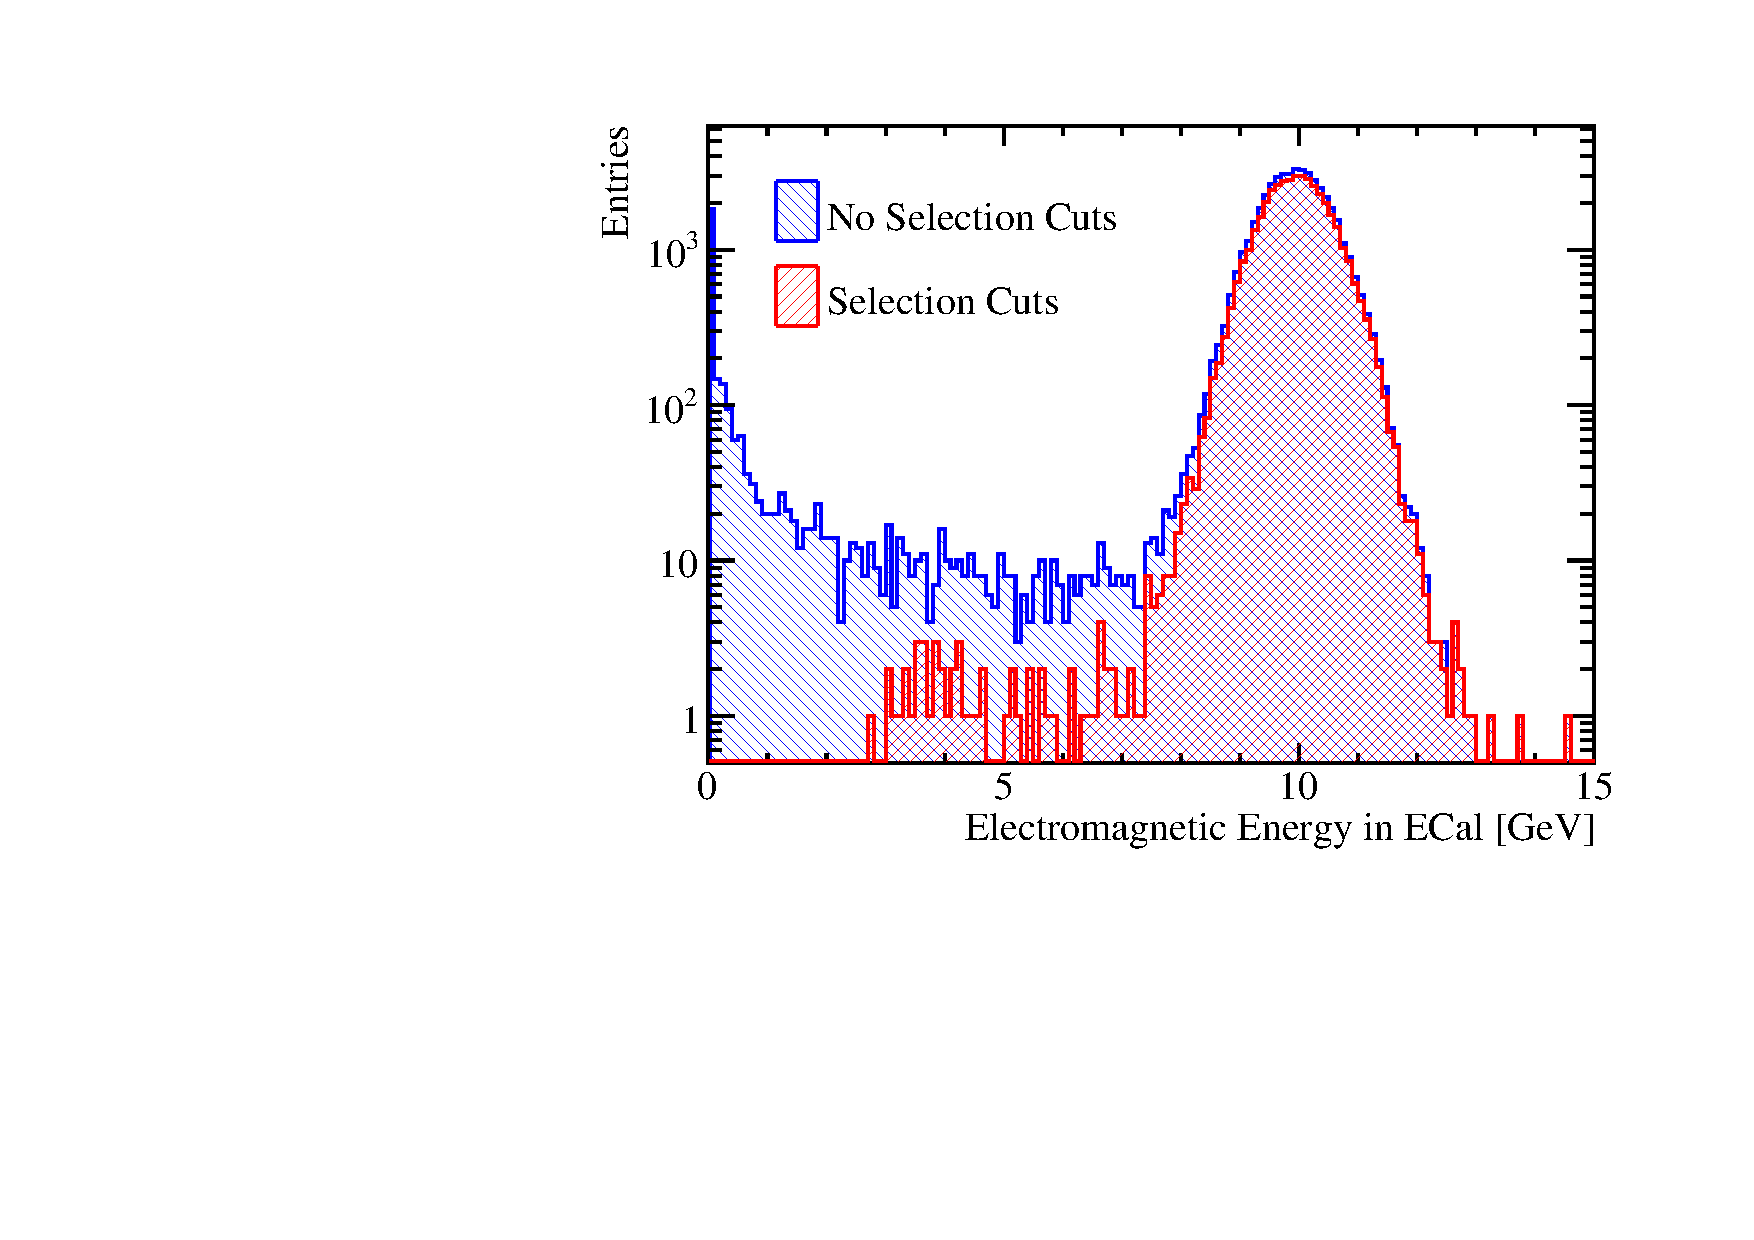
\includegraphics[width=0.5\textwidth]{Calibration/Plots/Calibration/EMScaleSetting/EMScaleECalSelection.pdf}}
\subfloat[]{\label{fig:ecalemscalefit}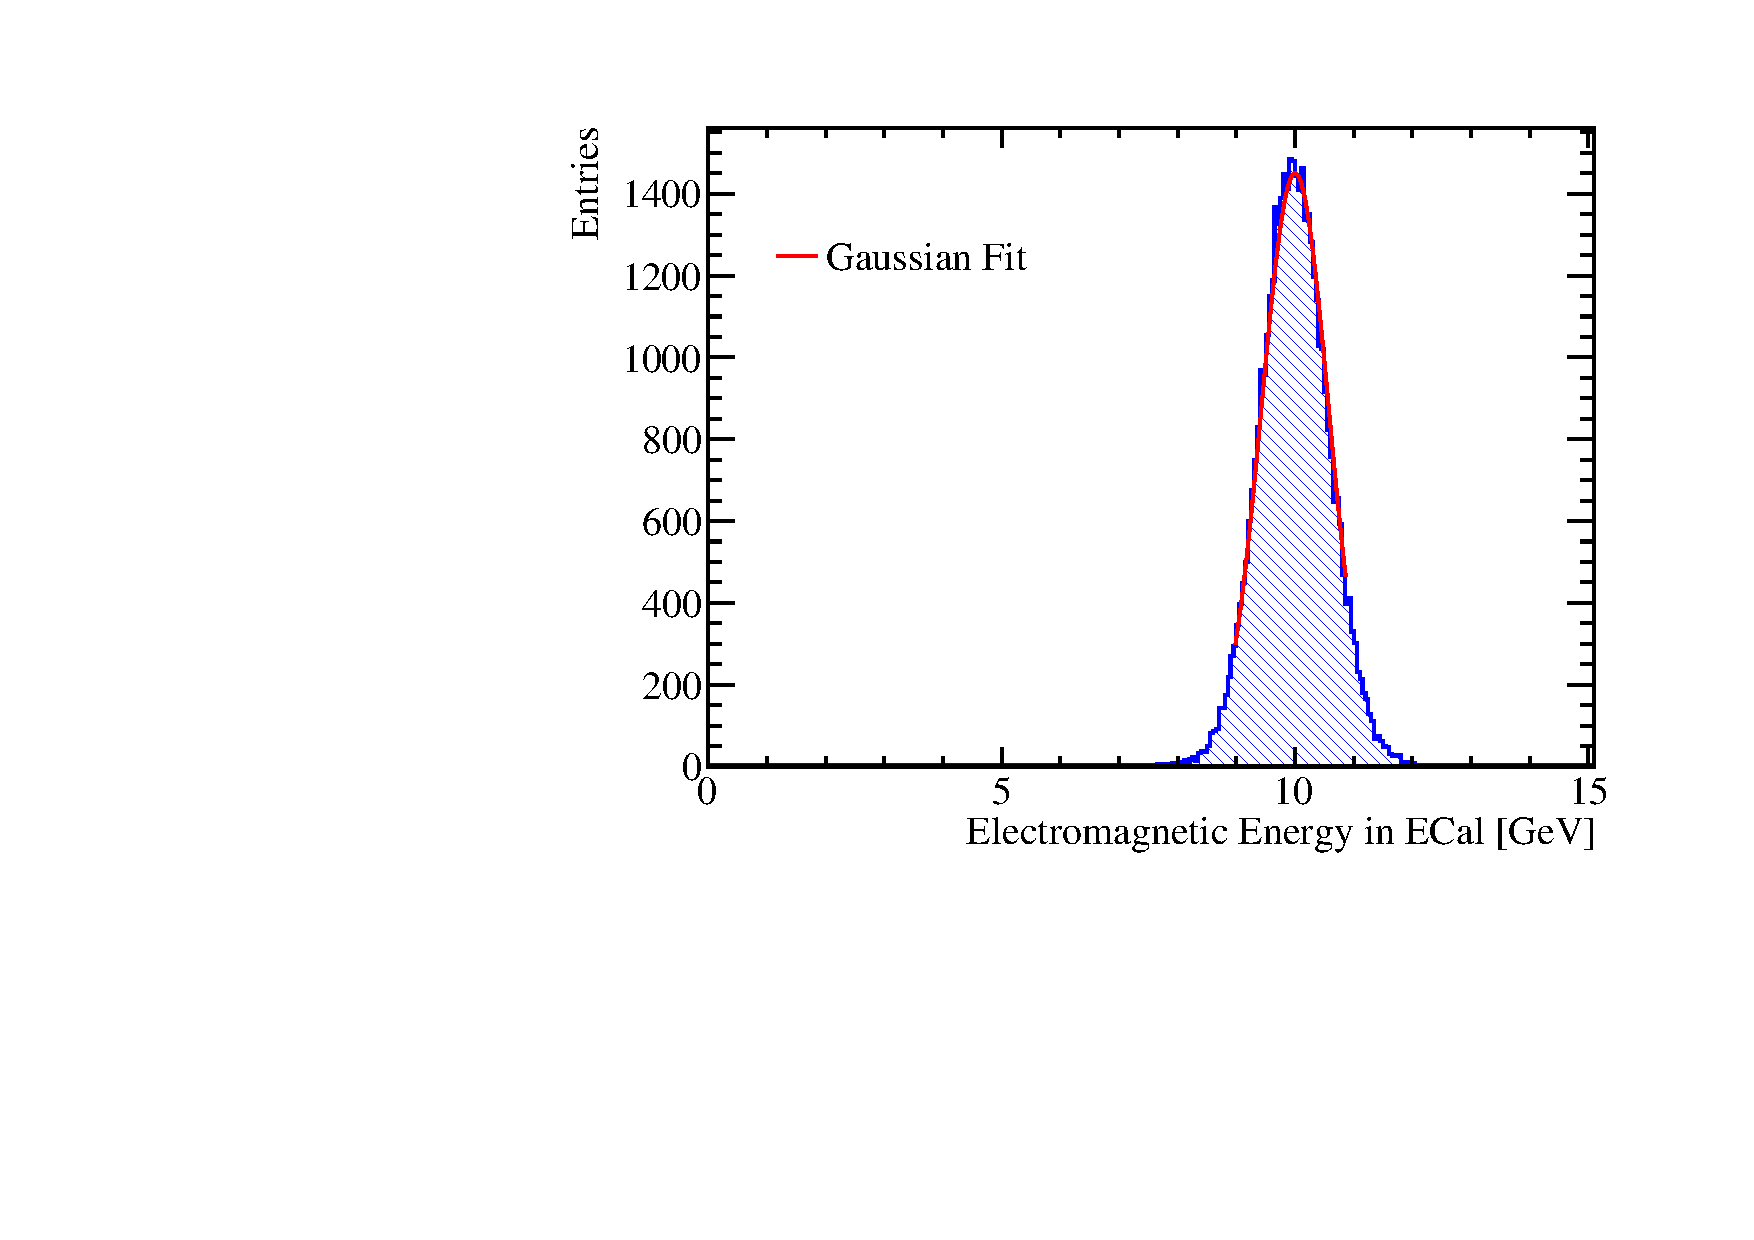
\includegraphics[width=0.5\textwidth]{Calibration/Plots/Calibration/EMScaleSetting/EMScaleSettingECalFit.pdf}}
\caption[\protect\subref{fig:ecalemscaleselection} The sum of the electromagnetic energy measured in the ECal for 10~GeV photons with and without the selection cuts.  \protect\subref{fig:ecalemscalefit} Gaussian fit to sum of the electromagnetic energy deposited in the ECal for 10~GeV photons with selection cuts.  The fine binning reflects the tolerance on the electromagnetic scale calibration constant in the ECal.]{\protect\subref{fig:ecalemscaleselection} The sum of the electromagnetic energy measured in the ECal for 10~GeV photons with and without the selection cuts.  \protect\subref{fig:ecalemscalefit} Gaussian fit to sum of the electromagnetic energy deposited in the ECal for 10~GeV photons with selection cuts.  The fine binning reflects the tolerance on the electromagnetic scale calibration constant in the ECal.}
\label{fig:ecalemscale}
\end{figure}
 
The electromagnetic scale in the HCal, $\beta^{EM}_{HCal}$, is chosen to be equal to the hadronic scale in the HCal, $\beta^{Had}_{HCal}$.  The details of the determination of $\beta^{Had}_{HCal}$ can be found in section \ref{sec:hadscalesetting}.  For the ILC and CLIC, $\beta^{EM}_{HCal}$ is not a critical parameter in the reconstruction as $\gamma$s are largely contained within the ECal meaning little to no electromagnetic energy is measured in the HCal.  

%========================================================================================

\subsubsection{Hadronic scale setting}
\label{sec:hadscalesetting}
The hadronic energy scale factors for the ECal and HCal, $\beta^{Had}_{ECal}$ and $\beta^{Had}_{HCal}$, are determined using $K^{0}_{L}$ events at $E_{MC} = 20$~GeV.  The hadronic scale in the ECal, $\beta^{Had}_{ECal}$, is important to detector performance as a non-negligible amount of hadronic energy will be measured in the ECal.  As the ECal contains $\approx 1 \lambda_{I}$, the hadronic scale in the ECal cannot be independently set as it is unfeasible to create a large sample of 20~GeV $K^{0}_{L}$ events that are fully contained within it.  Therefore, the hadronic scale in the ECal and HCal have to be set simultaneously.  

For the reasons outlined in section \ref{sec:hcaldigi}, the target reconstructed energy for this sample is the kinetic energy, $E_{K}$, of the $K^{0}_{L}$ as opposed to the total energy.  To ensure the events used are not affected by leakage of energy out of the back of the HCal, a cut is applied that vetoes events where energy is deposited in the outermost 10\% of the HCal.  In addition to this, a cut requiring a single neutral hadron to be reconstructed is applied to veto events with reconstruction failures.  Finally, it is required that the total hadronic energy measured within the calorimeters fall within three $\sigma$ of the kinetic energy of the $K^{0}_{L}$, where $\sigma$ is defined to be $55\% \times \sqrt{E_{K}}$~GeV.  This definition for $\sigma$ is approximately the energy resolution for neutral hadrons using the nominal ILD HCal \cite{Behnke:2013lya}.  This cut ensures that when fitting the two dimensional distribution of hadronic energy measured in the ECal and HCal outliers do not skew the fit.   The impact of cuts is illustrated in figure \ref{fig:hadscaleselection}.

\begin{figure}[h!]
\subfloat[]{\label{fig:hadscaleselectionnocuts}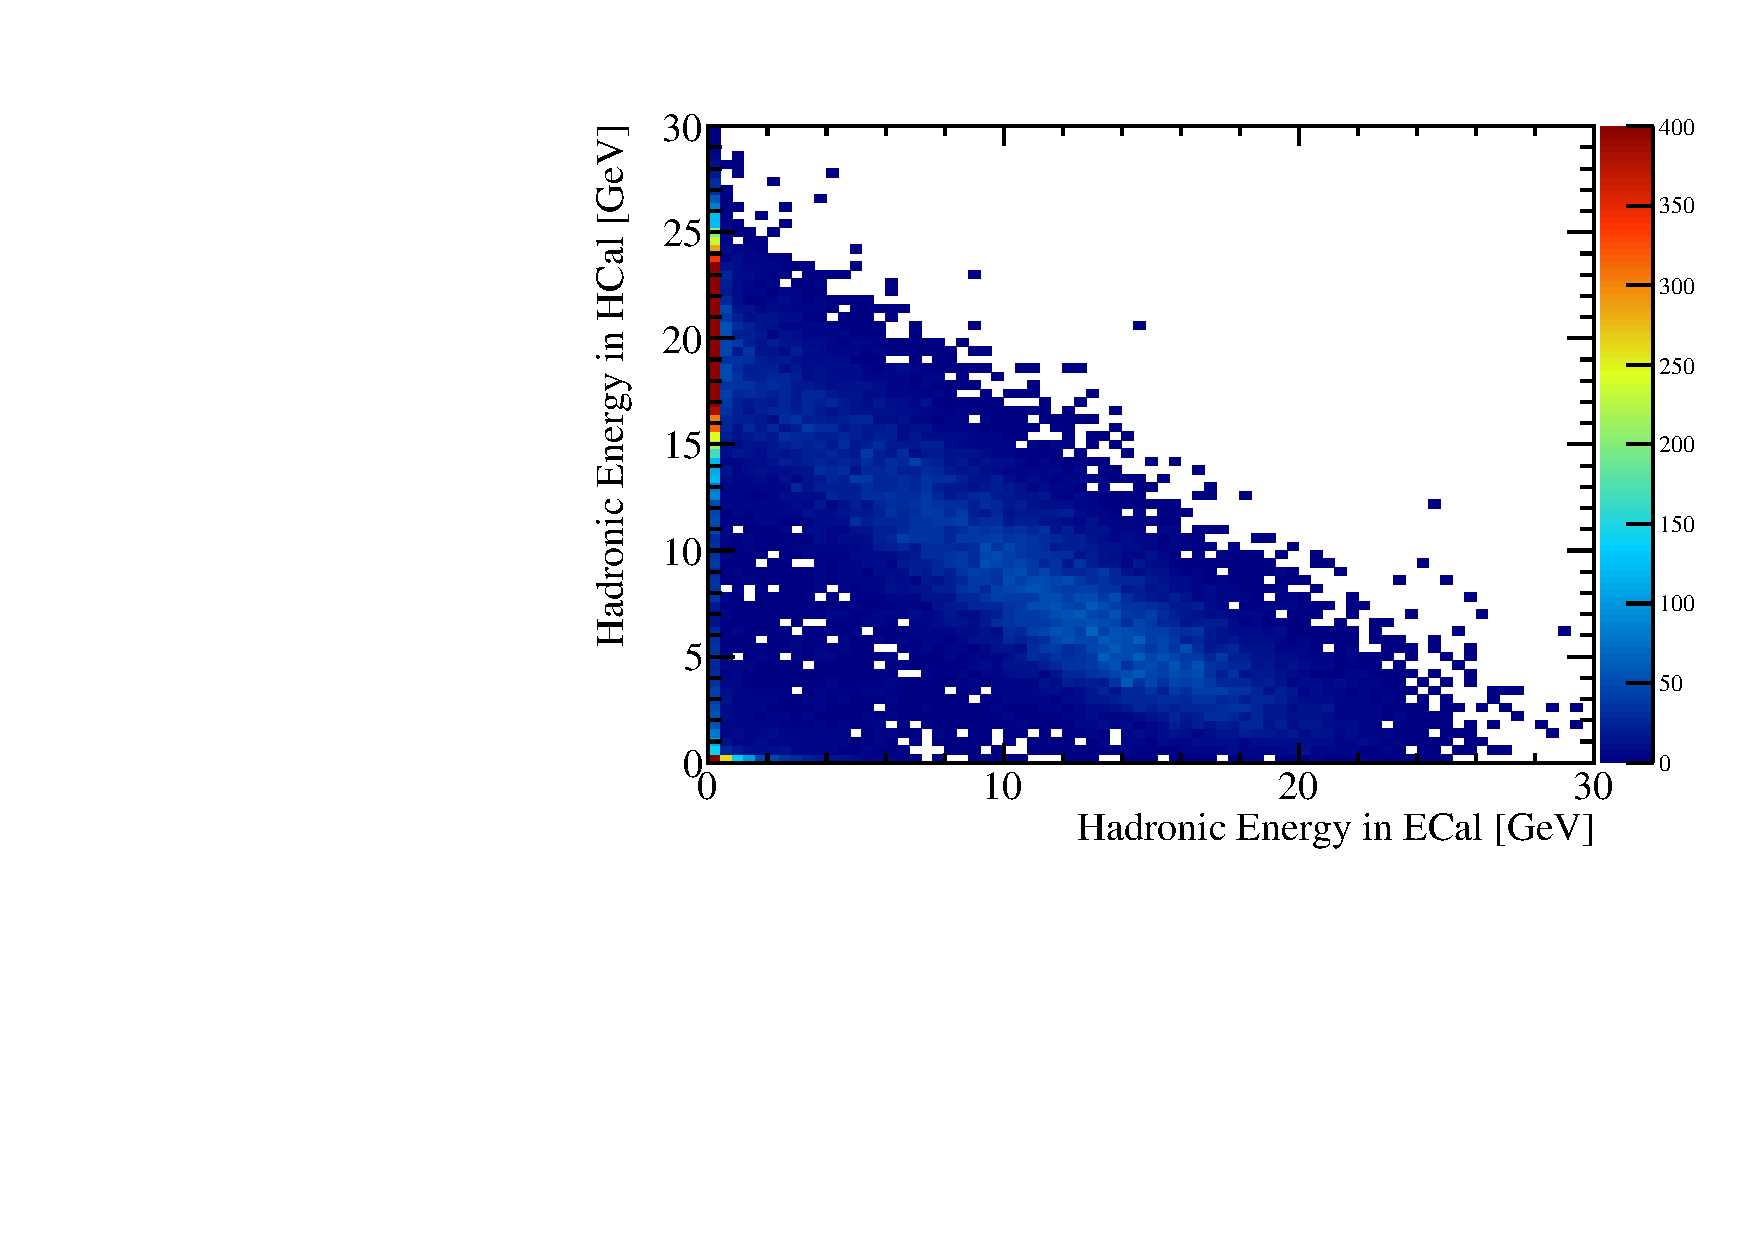
\includegraphics[width=0.5\textwidth]{Calibration/Plots/Calibration/HadScaleSetting/HadScaleECalHCalSelectionNoCuts.pdf}}
\subfloat[]{\label{fig:hadscaleselectioncuts}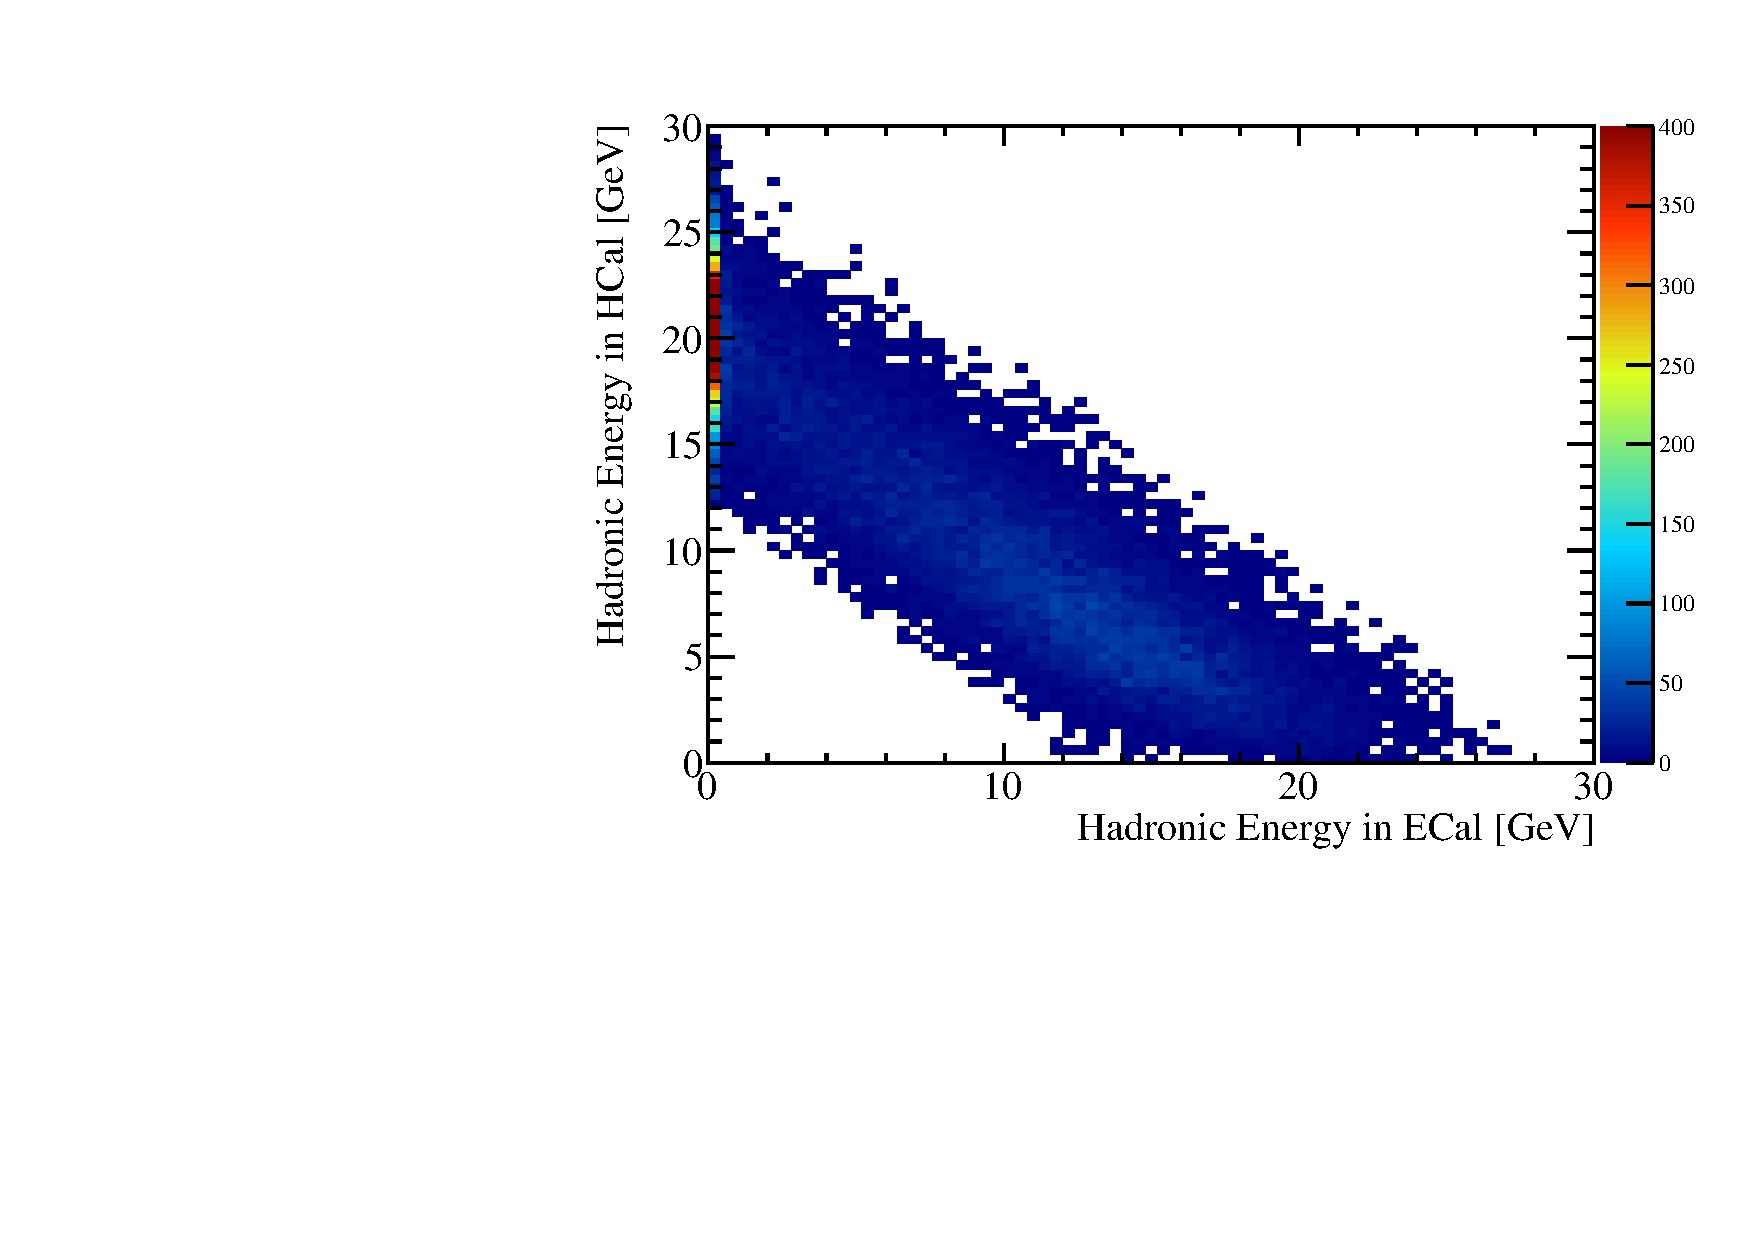
\includegraphics[width=0.5\textwidth]{Calibration/Plots/Calibration/HadScaleSetting/HadScaleECalHCalSelectionCuts.pdf}}
\caption[The distribution of hadronic energy measured in the ECal and HCal for 20~GeV $K^{0}_{L}$ events with and without selection cuts.]{The distribution of hadronic energy measured in the ECal and HCal for 20~GeV $K^{0}_{L}$ events \protect\subref{fig:hadscaleselectionnocuts} without selection cuts and \protect\subref{fig:hadscaleselectioncuts} with selection cuts.}
\label{fig:hadscaleselection}
\end{figure}

This part of the calibration procedure is again iterative and begins by assuming trial values, $\beta^{Had0}_{ECal}$ and $\beta^{Had0}_{HCal}$, for the hadronic scale calibration factors $\beta^{Had}_{ECal}$ and $\beta^{Had}_{HCal}$.  Following this the 20~GeV $K^{0}_{L}$ events are simulated and reconstructed using these scale factors.  Then a linear fit is applied to the two dimensional distribution of the reconstructed hadronic energies measured in the ECal and HCal for events passing the selection cuts.  The best fit is obtained by minimising $\chi^{2}$ with respect to variables describing a linear fit to the distribution.  In this case, $\chi^{2}$ is defined as
%
\begin{equation}
\chi^{2}(\delta^{Had}_{ECal}, \delta^{Had}_{HCal}) = \sum_{i} \frac{r_{i}}{\sigma_{r_{i}}}\text{ ,}
\end{equation}
%
\noindent where $r_{i}$ is the perpendicular distance in the two dimensional plane of hadronic energies measured in the ECal and HCal from the point $(x_{i}, y_{i})$ to a straight line passing through the points $(\delta^{Had}_{ECal}, 0)$ and $(0, \delta^{Had}_{HCal})$.  In this definition, $x_{i}$ and $y_{i}$ are the hadronic energies measured in the ECal and HCal respectively for event $i$.  The variables $\delta^{Had}_{ECal}$ and $\delta^{Had}_{HCal}$ describe a linear fit to the hadronic energy distribution, which are to be varied when minimising $\chi^{2}$.  The explicit definition of $r_{i}$ is given in equation \ref{equ:xicalc}, however it is best illustrated by considering figure \ref{fig:hadscalechi2calc}.  The uncertainty on $r_{i}$ is given by $\sigma_{r_{i}}$, which is explicitly defined in equation \ref{equ:sigmaxicalc}.  This uncertainty is calculated by propagating the uncertainties on $x_{i}$ and $y_{i}$, which are assumed to be $\sigma_{x_{i}/y_{i}} = 55\% \times \sqrt{x_{i}/y_{i}}$, into the expression for $r_{i}$.  The sum runs over all events, $i$, passing the selection cuts.  
%
\begin{equation}
r_{i} = \frac{y_{i} \delta^{Had}_{ECal} + x_{i} \delta^{Had}_{HCal} - \delta^{Had}_{ECal} \delta^{Had}_{HCal}}{\sqrt{(\delta^{Had}_{ECal})^{2} + (\delta^{Had}_{HCal})^{2}}}\text{ ,}
\label{equ:xicalc}
\end{equation}
\begin{equation}
\sigma_{i} = \frac{(\sigma_{y_{i}}  \delta^{Had}_{ECal})^{2} + (\sigma_{x_{i}} \delta^{Had}_{HCal})^{2}}{\sqrt{(\delta^{Had}_{ECal})^{2} + (\delta^{Had}_{HCal})^{2}}}\text{ ,}
\label{equ:sigmaxicalc}
\end{equation}
%
\begin{figure}[h!]
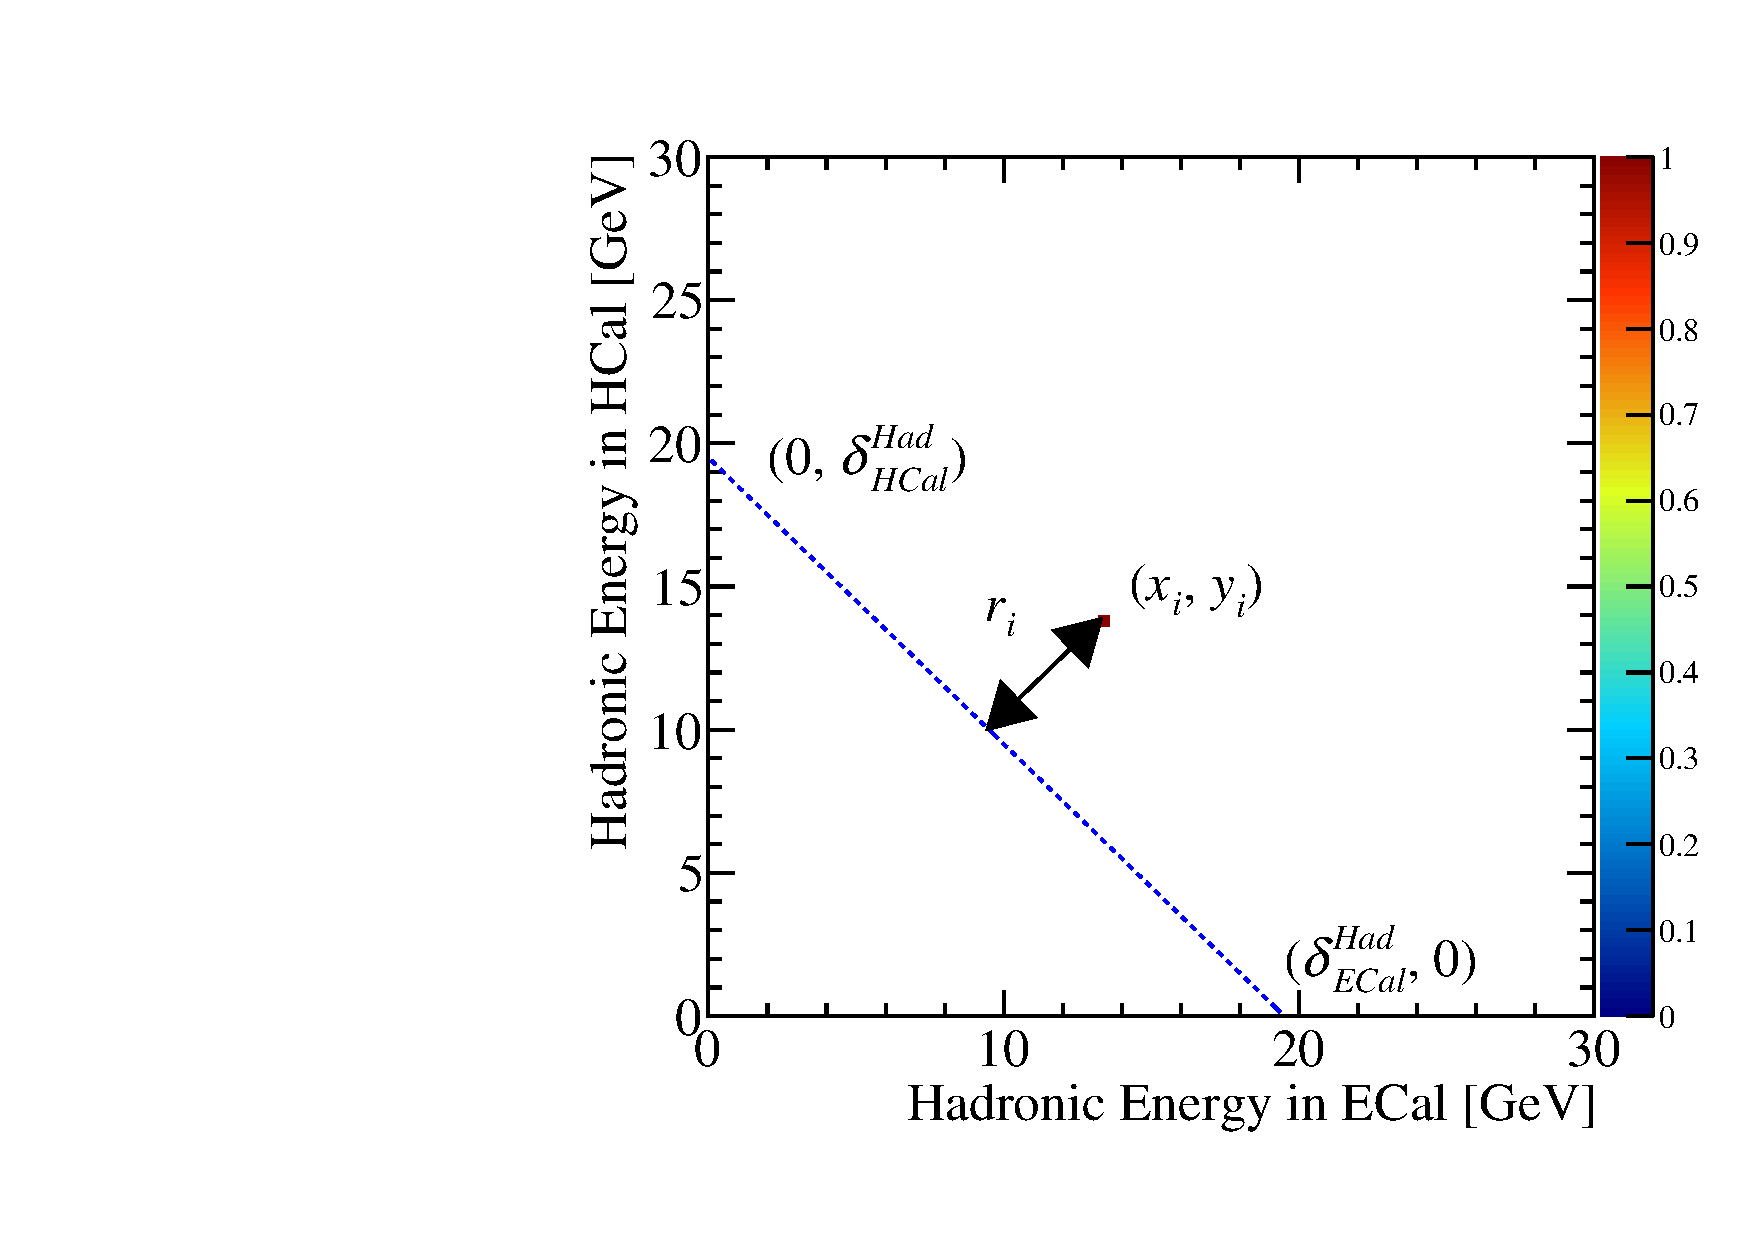
\includegraphics[width=0.5\textwidth]{Calibration/Plots/Calibration/HadScaleSetting/HadScaleECalHCalSelectionExample.pdf}
\caption[An example showing the definition of $r_{i}$, the variable used for the calculation of $\chi^{2}(\delta^{Had}_{ECal}, \delta^{Had}_{HCal})$ in determining the hadronic energy scale factors.]{An example showing the definition of $r_{i}$, the variable used for the calculation of $\chi^{2}(\delta^{Had}_{ECal}, \delta^{Had}_{HCal})$ in determining the hadronic energy scale factors.  For an event that has been measured with hadronic energy $x_{i}$ in the ECal and $y_{i}$ in the HCal, the geometric interpretation of $r_{i}$ is shown.  The blue dotted line is defined as $y_{i} = \delta^{Had}_{HCal} - x_{i} \frac{\delta^{Had}_{HCal}}{\delta^{Had}_{ECal}}$.}
\label{fig:hadscalechi2calc}
\end{figure}
%
\noindent The minimisation of $\chi^{2}$ is done by stepping over a range of $\delta^{Had}_{ECal}$ and $\delta^{Had}_{HCal}$ centred about the ideal value of $E_{K}$ in search for the minimum $\chi^{2}$.  Once the minima in $\chi^{2}$ is found the trial calibration factors $\beta^{Had0}_{ECal}$ and $\beta^{Had0}_{ECal}$ are rescaled to correct for any deviation from the desired fit as follows
%
\begin{equation}
\beta^{Had0}_{ECal} \rightarrow \beta^{Had}_{ECal} = \beta^{Had0}_{ECal} \times \frac{E_{K}}{\Delta^{Had}_{ECal}} \text{ ,}\\
\beta^{Had0}_{HCal} \rightarrow \beta^{Had}_{HCal} = \beta^{Had0}_{HCal} \times \frac{E_{K}}{\Delta^{Had}_{HCal}}\text{ ,}
\end{equation}
%
\noindent where $\Delta^{Had}_{ECal}$ and $\Delta^{Had}_{ECal}$ are the values of $\delta^{Had}_{ECal}$ and $\delta^{Had}_{ECal}$ giving the minimum $\chi^{2}$.  The step size used for minimising $\chi^{2}$ with respect to $\delta^{Had}_{ECal}$ and $\delta^{Had}_{ECal}$ was chosen such that a single step would correspond to the final tolerance on $\delta^{Had}$, which in this case is $\approx$ 0.1~GeV.  This procedure is then repeated using the updated hadronic scaling factors until $\Delta^{Had}_{ECal}$ and $\Delta^{Had}_{ECal}$ both fall within a specified final tolerance, which in this case it taken to be $|\Delta^{Had}_{E/HCal} - E_{\text{{K}}}| < E_{\text{{K}}} \times 0.5 \% \approx 0.1 \text{GeV}$.

%========================================================================================
%========================================================================================

\section{Conclusions}
Summarise this bit in a quick sentence.  After done calibration procedure, retrain...

\subsubsection{Photon Likelihood Data}
Some of the algorithms in PandoraPFA make use of likelihood data to identify electromagnetic showers.  This likelihood data consists of a series of probability density functions (PDFs) that describe a number of topological properties of PFOs.  The data contained in these PDFs is related solely to the ECal, which means that every time the ECal is changed from that of the nominal ILD detector this likelihood data must be retrained.  Should retraining be necessary it should be performed after the application of the calibration procedure as described in section \ref{sec:ordercalibration}.  To ensure PandoraPFA gives optimal performance for jet reconstruction, the likelihood data is trained using off-shell mass Z boson events, at 500~GeV, decaying into light quarks (u, d, s).  
